\chapter[Few-dipole Coupled Cavities]{Cavities with a Few Discrete Dipoles}\label{ch:cavity}


%%%%%%%%%%%%%%%%%%%%%%%%%%%
In the first section of this chapter, we will numerically demonstrate the GFTs and spectra for a H3 PC cavity with a small number of dipoles. How the physical parameters affect the spectral lineshape and resonances will be discussed. Different calculation methods will be checked.
The cross-coupling effect of different components of GFT will also be discussed in this chapter.
As will be shown later in this chapter,
the cross-coupling effect between different polarization components may be weak,
but it exists.
%so that one can focus on one-direction polarized spectrum to study the cavity property with an ensemble of dipoles, as will be discussed in Chapter~\ref{ch:ensemble}.

In the second section of this chapter, the spectrum of the PC cavity with $41$ discrete dipoles will be studied using the computation method verified in the first section of this chapter. It will demonstrate the impaction of frequencies repulsion effect and increasing coupling strength, as they are important for the discussions in the next chapter.

%I would also like to address that micropillar cavity, which has an almost evenly distributed field with a high symmetry in all directions may exhibit considerable cross-coupling effect between different polarization directions. Because of lack of time, this guess is listed as a future work in Chapter~\ref{ch:Conclusion}.

\section[One- and Two-dipole Coupled Cavities]{One- or Two-dipole coupled Cavities}
%\subsection{One-dipole Coupled PC Cavity}
We have three aims in this section. One is to verify our computational algorithms; one is to discuss the nature of the spectra and the movements of various peaks; another is to observe the cross-coupling effect, and to reveal the limitation of the 1-D model to inspire a future work.

To verify an algorithm, it is better to compare the calculation results of the algorithm with standard or published results. We have three algorithms for the GFTs calculation: the first one is called the iterative method based on iterative Dyson equations; the second one is called the non-iterative method, based on inverting of large matrix (see Appendix~\ref{App:GF}); the last one is based on the method described in Appendix~\ref{section:GFscalar}. We temporarily call it the scalar algorithm, which projects tensors and vectors onto the dipoles vectors and makes scalar algebra suitable for some cases. The iterative algorithm is based on the idea that every time a dipole added into a cavity the GF will be changed based on the Dyson equation. It requires less computer resources, and hence suitable for dense dipoles coupled cavities calculation. The non-iterative algorithm can calculate the total GF including many dipoles at once. It requires a large computer memory, and fails to calculate if the number of dipoles is too large to be handled with limited computational resources. The last algorithm is based on the idea that only the quantities (GFs or E-field) projected in the dipole oscillation direction matter to the spectrum. It also requires a large memory to calculate. We will use the projection idea to show that, if we only project the GF to the $y$-direction rather than the actual dipole oscillation direction, the cross-coupling effect occurs.
%
%In our study, the non-iterative method is expected to be used for computation accuracy correction, since the non-iterative method has less iterative errors compared to the iterative method. And we find that the computational errors of both non-iterative and iterative algorithms are very close for considerable $N$, and the non-iterative algorithm is not suitable for the computation task of large $N$ case. Therefore, the non-iterative algorithm is not presented in this section.

The published formulas and our studying steps for one- and two-dipole coupled cavities are listed as follows.

{\textbf 1.} We will check our result for the one-dipole case with reference~\cite{Hughes2009}. For the on-resonance strongly coupling case, we should get a doublet. The splitting width should be $w_1=2g=2\times\sqrt{\frac{\omega_o}{2\hbar \varepsilon_0}}\boldsymbol{\mu}_1\cdot \mathbf{f}_y(\mathbf{r}_1)=2\times0.55411$ meV. I used the following analytical spectrum formula to check against the result directly obtained from our Dyson iteration code. The published formula is given by~\cite{Hughes2009}
\begin{equation}
 S_{cav}=C\cdot \left| \frac{2g\omega_0(\omega+\omega_1)}{(\omega^2-\omega_1^2+i\omega \Gamma_1)(\omega^2-\omega_0+i\omega \Gamma_y)-4g^2\omega_y \omega} \right|^2,
\label{spec_1dot}
\end{equation}
where $C$ is a geometric factor depending on the detector location and effective exciton decay rate. $C$ does not change the shape and position of the spectrum, so we treat it as a constant. To make a good comparison, we use a H3 PC cavity to define a given distribution of field, and adapt the other parameters to those reported in Ref.~\cite{Hughes2009}.

{\textbf 2.} We will check a two-dipole system with reference~\cite{Yao2009c}. If we put both dipoles on-resonance, a broadened doublet will be observed. An explicit expression for $\mathbf{G}^2(\mathbf{r},\mathbf{r}_a,\omega)$ is given by~\cite{Yao2009c}
\begin{equation}
 \label{G2}
\mathbf{G}^2(\mathbf{r},\mathbf{r}_a,\omega)=\frac{\mathbf{G}_1^1(\mathbf{r},\mathbf{r}_a,\omega)+\mathbf{G}^1_1(\mathbf{r},\mathbf{r}_b,\omega)\cdot \boldsymbol{\alpha}_b(\omega)\cdot \mathbf{G}^1_1(\mathbf{r}_b,\mathbf{r}_a,\omega)}{1-\mathbf{G}^1_1(\mathbf{r}_a,\mathbf{r}_b,\omega)\cdot \boldsymbol{\alpha}_b \cdot \mathbf{G}^1_1(\mathbf{r}_b,\mathbf{r}_a,\omega)\cdot \boldsymbol{\alpha}_a(\omega)},
\end{equation}
where
\begin{equation}
 \label{tildeG}
\mathbf{G}^1_1(\mathbf{r},\mathbf{r}_m,\omega)=\frac{\mathbf{G}^0(\mathbf{r},\mathbf{r}_m,\omega)}{1-\mathbf{G}^0(\mathbf{r}_m,\mathbf{r}_m,\omega)\cdot \boldsymbol{\alpha}_m(\omega)},
\end{equation}
and $a,\, b, \, m=1,2$ are indexes of dipoles.

The physical content of the spectra will be discussed in the one- and two-dipole coupled PC cavity cases.

{\textbf 3.} To examine the cross-coupling effect, we will compare a diagonal element, $yy$-component, of the GFT calculated from the full tensor iterative algorithm with a full scalar algorithm which only take the $y$ component of the dipole moment and the $yy$ component of the bare cavity GFT into account. The difference of these two results is determined by the relative amplitude of $xy$ and $yx$ components of the GFTs to the diagonal elements, and indicates how large the $x$-$y$ components cross talk to each other. As will be shown shortly, the cross-coupling effect exists when the field and the dipole moment are not in the same direction. This effect may be important to discuss spin and polarization phenomena, but we will not cover this effect in the model discussed in Chapter~\ref{ch:ensemble}.

%Notice that, at the time of my writing this thesis, I could not redo the drawing work based on FDTD calculation. I can only find several early figures in my old documents may suitable for this section. Some plots have tiny labels which are difficult to recognize. I will provide detailed descriptions in the captions. There are two issues on the cavity mode figures presented in this section: one is that the $x$ and $y$ axes are defined differently from the next section; the field vectors plotted in this section is defined to be orthogonal to that in the next section. Since both of the above issues are caused by definition of coordinates when the mode distribution is plotted, and the conclusions regarding GFTs and spectra are correct and independent of notations, I use the old plots in this section as it was. I plead your pardon at this moment.
%The results are as follows.

\subsubsection{One-dipole cavity system with a y-polarized source}
This part mainly focuses on one-dipole coupled PC cavity system with the same parameters as that of reference~\cite{Hughes2009}.
%The testing code is located at GFT tool box repository/Test with the name SpecPC\_1.m (version 7).
The parameters in use are listed below:
%\begin{equation}
\begin{align}
 \omega_c/2\pi &= 317 {\text {THz}}\quad \quad (\lambda_c=945 {\text {nm}}),\\
 \Gamma_c &= 0.1 {\text {meV}}, \\
 g &= 0.1 {\text {meV}}, \\
 \Gamma_{d} &= 2 \mu{\text {eV}}
 \quad or\quad 40 \mu{\text {eV}},
\nonumber
\end{align}
%\end{equation}
where $\Gamma_{d}$ with two values is the decay rates the of dipole for 2 cases. The dipole is oriented along the y-axis, and is at the center of the cavity, or $\br_1=[0,\,0,\,0]$ nm (Fig.~\ref{dotsmode1_1}). We use the normalized mode of a full size H3 PC cavity~\cite{Hughes2009} (Fig.~\ref{dotsmode1_1}), so that the optical moment of the dipole ($\approx 41 \text{Debye}$) can be obtained through solving the equation
\begin{equation}\label{eq:g1}
g=\sqrt{\frac{\omega_o}{2\hbar \varepsilon_0}}\boldsymbol{\mu}_{1}\cdot \mathbf{f}_y(\mathbf{r}_{1}).
\end{equation}
The subscript ``$y$'' of $\mathbf{f}_y(\mathbf{r}_{1})$ indicates that we only considered the y-mode of the cavity.

Since our dipole source is orientated in the y direction, and the y component of the cavity mode dominates the field, the yy component of GFT should dominate all physical effects. Scalar analysis only using the yy component of the bare cavity GFT should give the same result as the full tensor calculation with the GFT. Below is the result. The background GFT for this cavity is shown in Fig.\ref{G84_11_1}.

By putting dipole 1 at the center of the cavity (see Fig.\ref{dotsmode1_1}), the GFT components including one dipole, either on- or off-resonance, are illustrated in Figs.~\ref{G84_yy11_1} and~\ref{G84_1yy_1}. It shows that the detecting position does not affect the shape of GF. The spectra of two off- and on-resonance dipoles cases are shown in Figs.~\ref{sp84_11_1} and~\ref{sp84_11_2}.

For the off-resonance cases, the decay rates determine the linewidth of the exciton peak, and the relative amplitude of the cavity peak. The narrower is the exciton peak, the smaller the cavity peak, relative to the maximum value of the peaks. The closer the exciton approaches to the cavity resonance, the larger the cavity peak will become (not shown here). We also notice that there is a small shift of the exciton peak position, relative to the intrinsic value, $\Omega_d$. This can be explained by the fact that each peak of the two is summed with the inclined spectral tail of the other peak, and the inhomogeneous summation over frequencies shifts the peaks away from each other in the frequency domain. We call this effect the ``repulsion'' effect. We will discuss this effect in-depth in the next section.

For the on-resonance cases, the cavity spectrum is basically unchanged with various exciton decay rate ($<\Gamma_c$). In the strong coupling regime, doublets occur as a result of Rabi oscillation, in which the exciton and the cavity exchange energy back and forth long-lastly and form dressed states with a large energy splitting~\cite{Scully1997,Qi2011d}. The decay rate of the exciton can affect the depth of the dip between the doublets; while the width of the splitting approximates to $2g$, and is mainly determined by the coupling strength. For example, in Fig.~\ref{sp84_11_2}, both cases of $\Gamma_d=2\mu eV$ and $40\mu eV$ give the same splitting width $\approx 0.0947$ meV $\lesssim 2g$; the lowest point in the dips of the two cases (from top to bottom) are at $0.1215$ and $0.1982$ units relative to the maximum of the doublets. Once there are doublets in the spectrum, there are also doublets in the imaginary part of the total GFT elements. In general, the peaks in the total GFT elements correspond to the peaks in the spectrum. This correspondence may not hold if there are multi large components of the GFTs or the GFTs with multi emitting sources.


\begin{figure}[H]
\centering
\begin{center}
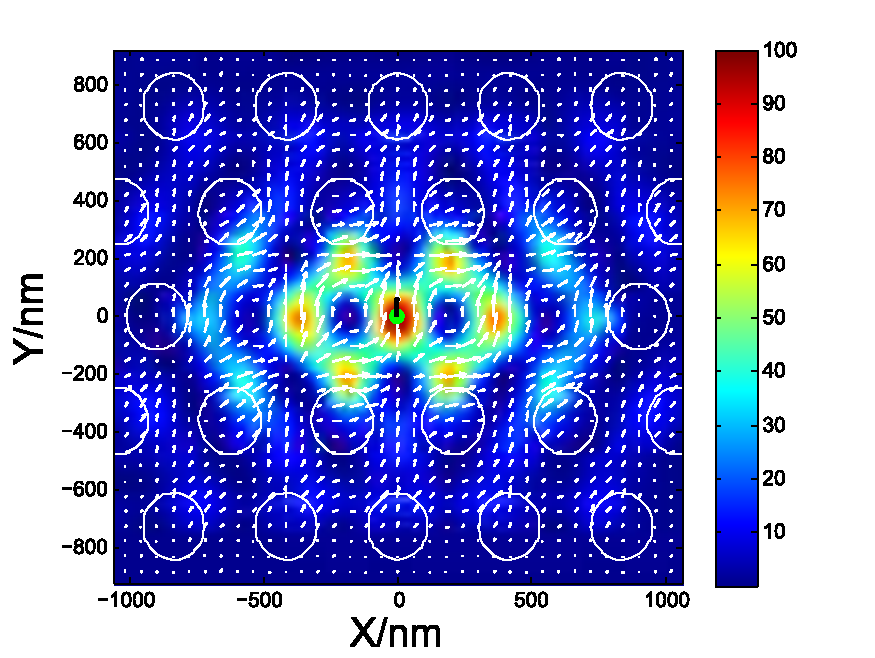
\includegraphics[width=16cm]{./Figs/dotsmode1_1}
\end{center}
\caption[Dipole and E-field distributions in a H3 PC cavity structure.]{\textbf{   Dipole and E-field distribution in a H3 PC cavity structure in the $z=0$ plane.}  The dipole (the green point) is polarized in y direction (see the black arrow) and is located at $[0,\, 0,\, 0]$ nm, which is the center of the cavity, with a strong y-polarized field. Color map and white arrows indicate relative strength and direction of the cavity field.}
\label{dotsmode1_1}
\end{figure}

\begin{figure}[H]
%\fontsize{18}{19}\selectfont
\centering
\begin{center}
%\psfrag{(w-w0)/meV}{$(\omega-\omega_c)/meV$}
\psfrag{realG}{real$\bG$}
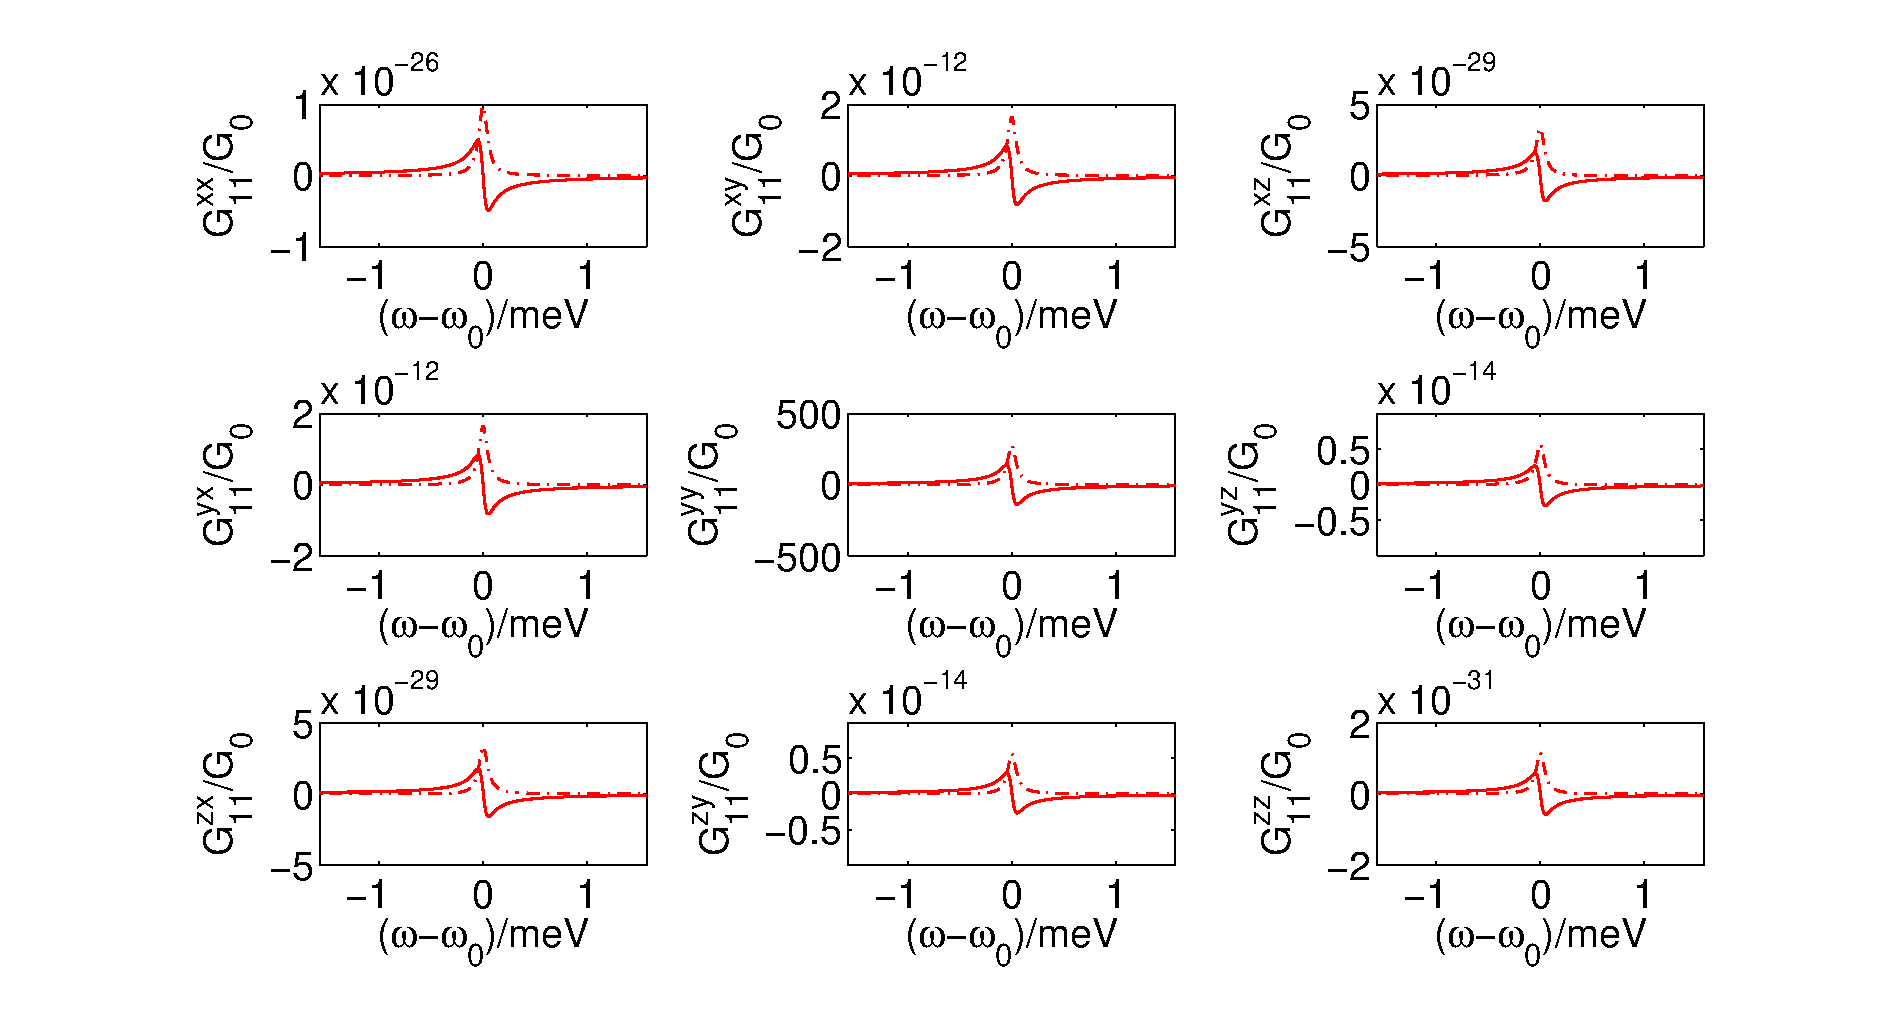
\includegraphics[width=16cm]{./Figs/G84_11_1}
\end{center}
\caption[Diagram of GFT tensor elements.]{\textbf{Full elements of $\mathbf{G}^0$ with $\omega_c/2\pi = 317 {\text {THz}}, \Gamma_c = 0.1 {\text {meV}}$ }. The $\mathbf{G}^{ij}_{11}$ is the $ij$-th component of the $\mathbf{G}^{(0)}(\br_1,\br_1,\omega)$. Dashed lines are the imaginary parts of the GFs; solid lines are the real parts of the GFs. All components are normalized to the homogeneous GF, $G_0$, given by Equ.\eqref{Ghom2}. As it shows, the $yy$ component dominates the GFT components.}
\label{G84_11_1}
%\normalsize
\end{figure}

\begin{figure}[H]
\centering
\begin{center}
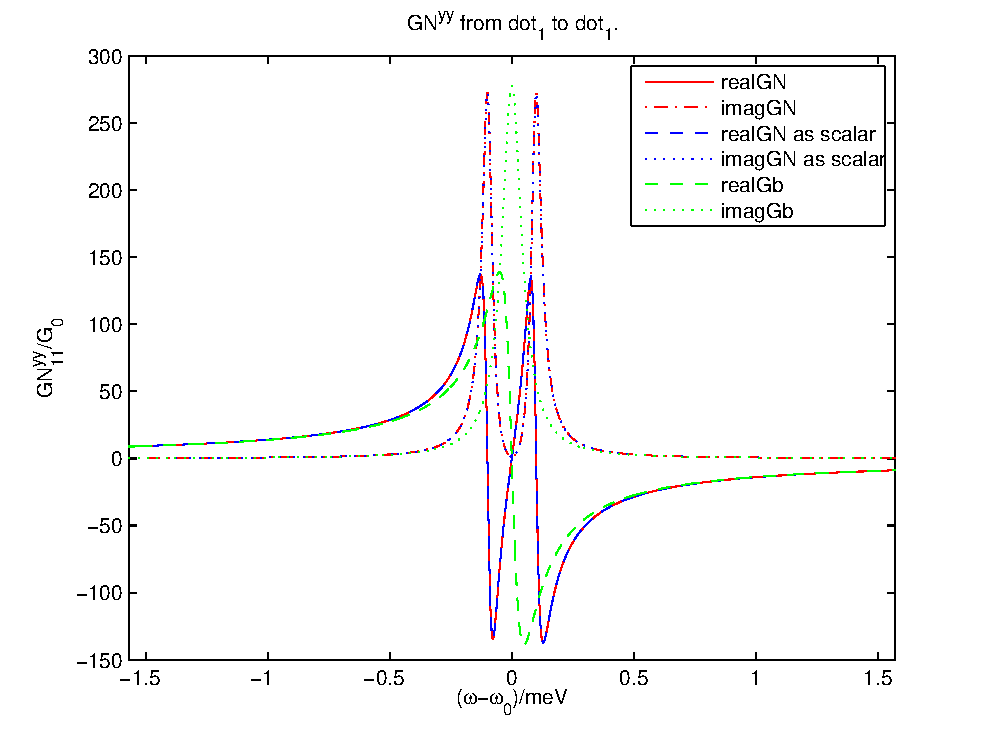
\includegraphics[width=14cm]{./Figs/G84_yy11_1}
\end{center}
\caption[yy component of $G^1(\mathbf{r}_1,\mathbf{r}_1)$ with an on-resonance dipole.]{\textbf{  yy component of $\mathbf{G}^1(\mathbf{r}_1,\mathbf{r}_1)$ with an on-resonance dipole of $\omega_d/2\pi = 317 {\text {THz}}, \Gamma_d = 2 \mu{\text {eV}}$ }. Red line shows the result calculated through full tensor iteration method; blue line is obtained by only considering y component of vectors through scalar iteration method; green line is bare cavity GF (yy-component) for comparison. Except for the bare cavity GF, all the other lines match up perfectly.}
\label{G84_yy11_1}
\end{figure}

\begin{figure}[H]
\centering
\begin{center}
\psfrag{dot}{dipole}
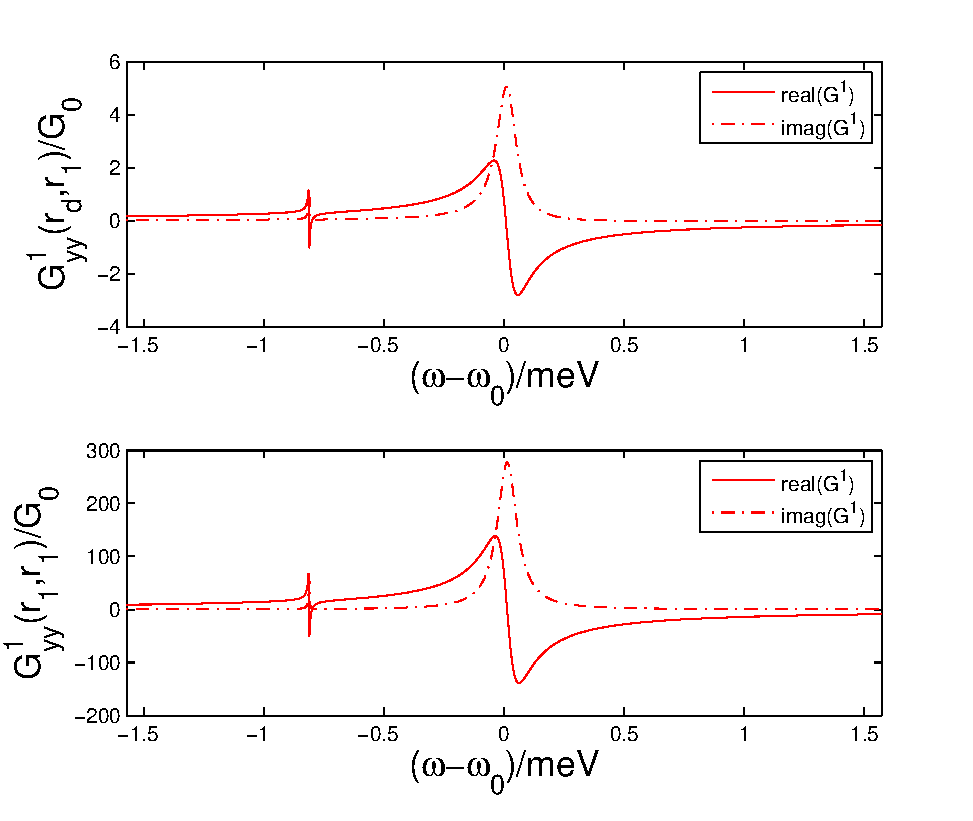
\includegraphics[width=14cm]{./Figs/G84_1yy_1}
\end{center}
\caption[yy component of GFT with an off-resonance dipole.]{\textbf{The yy components of $\bG^1(\mathbf{r}_d,\mathbf{r}_1)$ and $\bG^1(\mathbf{r}_1,\mathbf{r}_1)$  with an off-resonance dipole of $\Delta \omega = -0.8 {\text {meV}}, \Gamma_d = 2 \mu{\text {eV}}$ }. The upper plot shows the yy component detected at $\br_d=[0,\,0,\,420]$ nm above the cavity center; the bottom plot shows the yy component at the dipole responding to itself. Solid lines are the real parts of GFs. Dashed lines are the imaginary parts. }
\label{G84_1yy_1}
\end{figure}


\begin{figure}[H]
\centering
\begin{center}
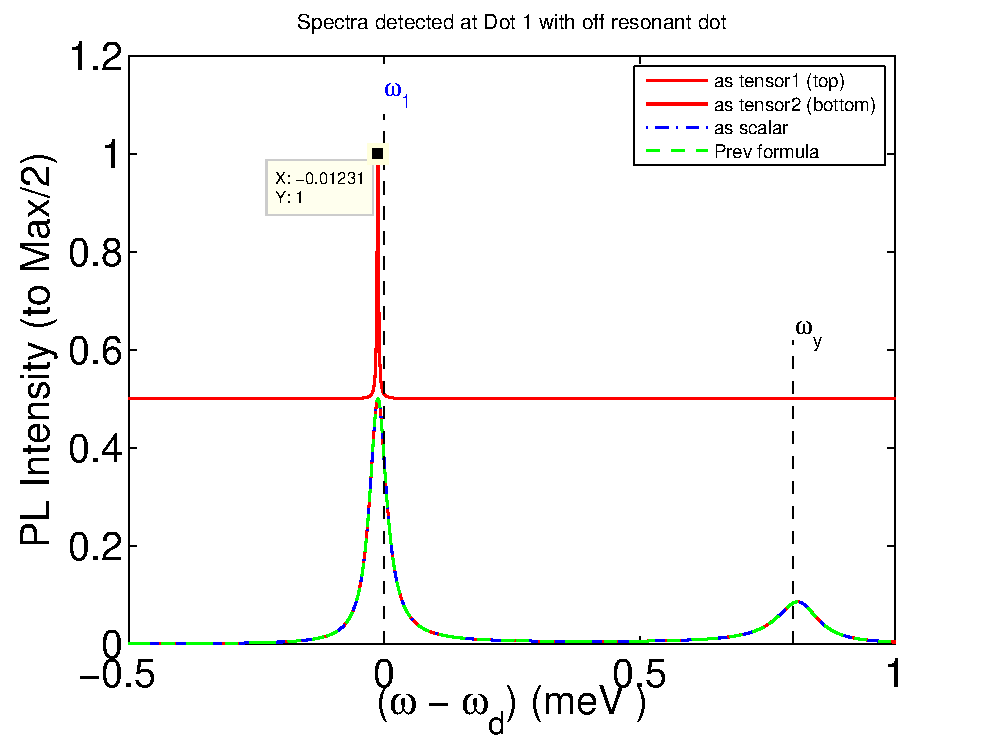
\includegraphics[width=14cm]{./Figs/sp84_11_1}
\end{center}
\caption[Spectra of off-resonance dipole in a PC cavity.]{\textbf{Spectra of off-resonance dipole in a PC cavity detected at the dipole position. $\Delta \omega = -0.8 {\text {meV}}$ }. $\omega_d$ is the dipole resonance; $\omega_y$ is the cavity resonance. $\Gamma_d = 2 \mu{\text {eV}}$ is used for the top plot; the bottom plot is with $\Gamma_d = 40 \mu{\text {eV}}$. For the bottom plot, the red, blue and green lines are obtained through full tensor method, scalar method (by only taking y component of dipole moment and $yy$ component of $\Gb$ into account) and according to the spectrum analytical formula given by Ref.~\cite{Hughes2009}. These three lines match up perfectly. The upper curves have be offset vertically by 0.5 for clarity. }
\label{sp84_11_1}
\end{figure}


\begin{figure}[H]
\centering
\begin{center}
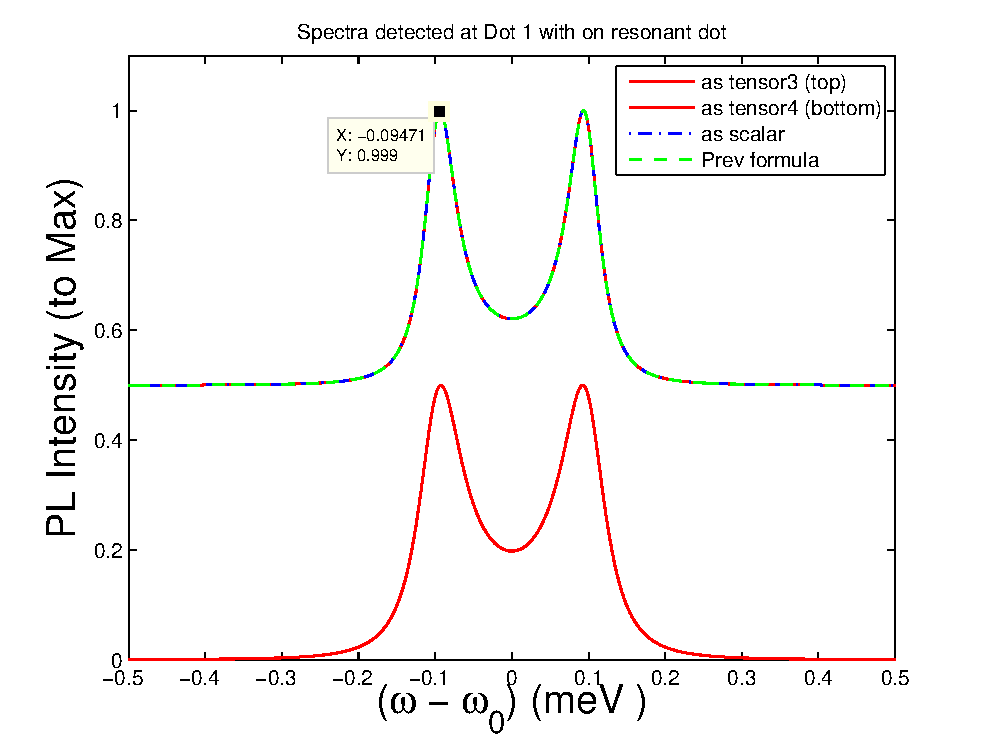
\includegraphics[width=14cm]{./Figs/sp84_11_2}
\end{center}
\caption[Spectra of a PC cavity with an on-resonance dipole.]{\textbf{Spectra of a PC cavity with an on-resonance dipole detected at the dipole position. $\Delta \omega = 0 {\text {meV}}$ }. Top lines are with a dipole decay rate of $\Gamma_d = 2 \mu{\text {eV}}$; bottom line is with $\Gamma_d = 40 \mu{\text {eV}}$. Notations are the same as Fig.~\ref{sp84_11_1}. Again, these three lines match up perfectly. There is an offset for 0.5 in the top curves for clarity.}
\label{sp84_11_2}
\end{figure}

\clearpage

\subsection{Cavity System with One $xy$-polarized Dipole}
As in the previous section, we still concentrate on one-dipole coupled cavity system,
but let us turn the dipole source's polarization direction at $45^\circ$ to the $x$ axis,
which means the polarization direction is between the $x$ and $y$ axes.
Now, the spectrum formula given by Ref.~\cite{Hughes2009} does not work for this case.
To further check the validity of the formula for the Green function in \cite{Hughes2009},
let us locate the dipole source at a place where both x and y components of the E-field contribute to the cavity GFT,
which leads to a ``non-diagonal'' GFT as a result.
And in this case, we cannot only use $yy$ component of GFT to analyze the spectrum.
%All graphs in this section are returned from code SpecPC\_1.m version 13 in Test file of GFT project repository.

The dipole location and polarization direction is shown in Fig.\ref{dotsmode1_2}
\begin{figure}[H]
\centering
\begin{center}
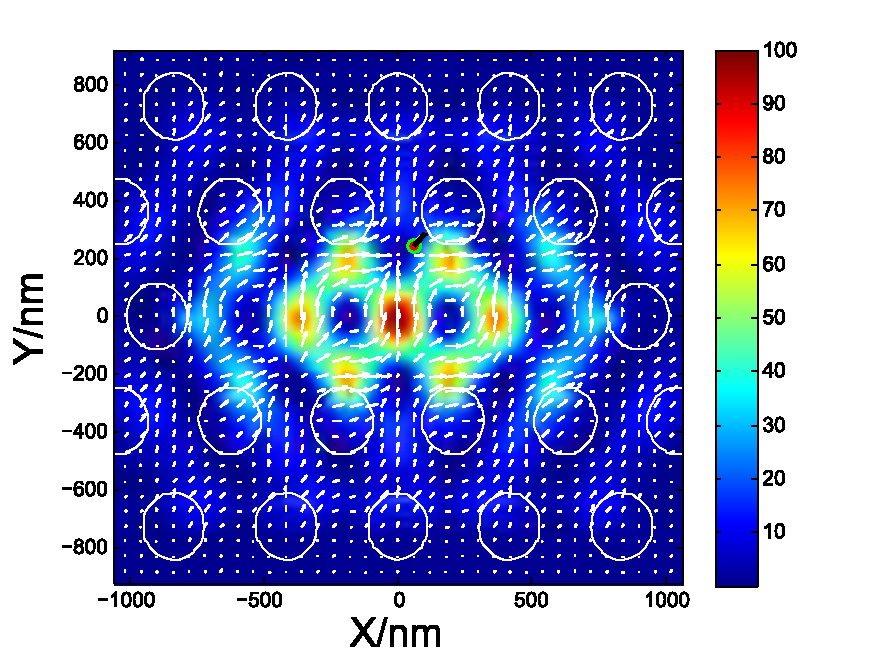
\includegraphics[width=14cm]{./Figs/dotsmode1_2}
\end{center}
\caption[Dipole and E-field distributions in a H3 PC cavity structure.]{\textbf{  Dipole and E-field distribution in a H3 PC cavity structure in $z=0$ plane.}  The dipole (indicated by the red point) polarizes in the x-y direction (see the black arrow at the dipole) and is located at $[60,100\times\sqrt{3}+60,\, 0]$ nm, where the E-field of the cavity has both x and y components. The color map corresponds to the relative strength of the cavity mode, and white arrows indicate on-site E-field vectors.}
\label{dotsmode1_2}
\end{figure}
The GFT elements for this bare cavity are shown in Fig.\ref{G84_11_4}.
\begin{figure}[H]
\centering
\begin{center}
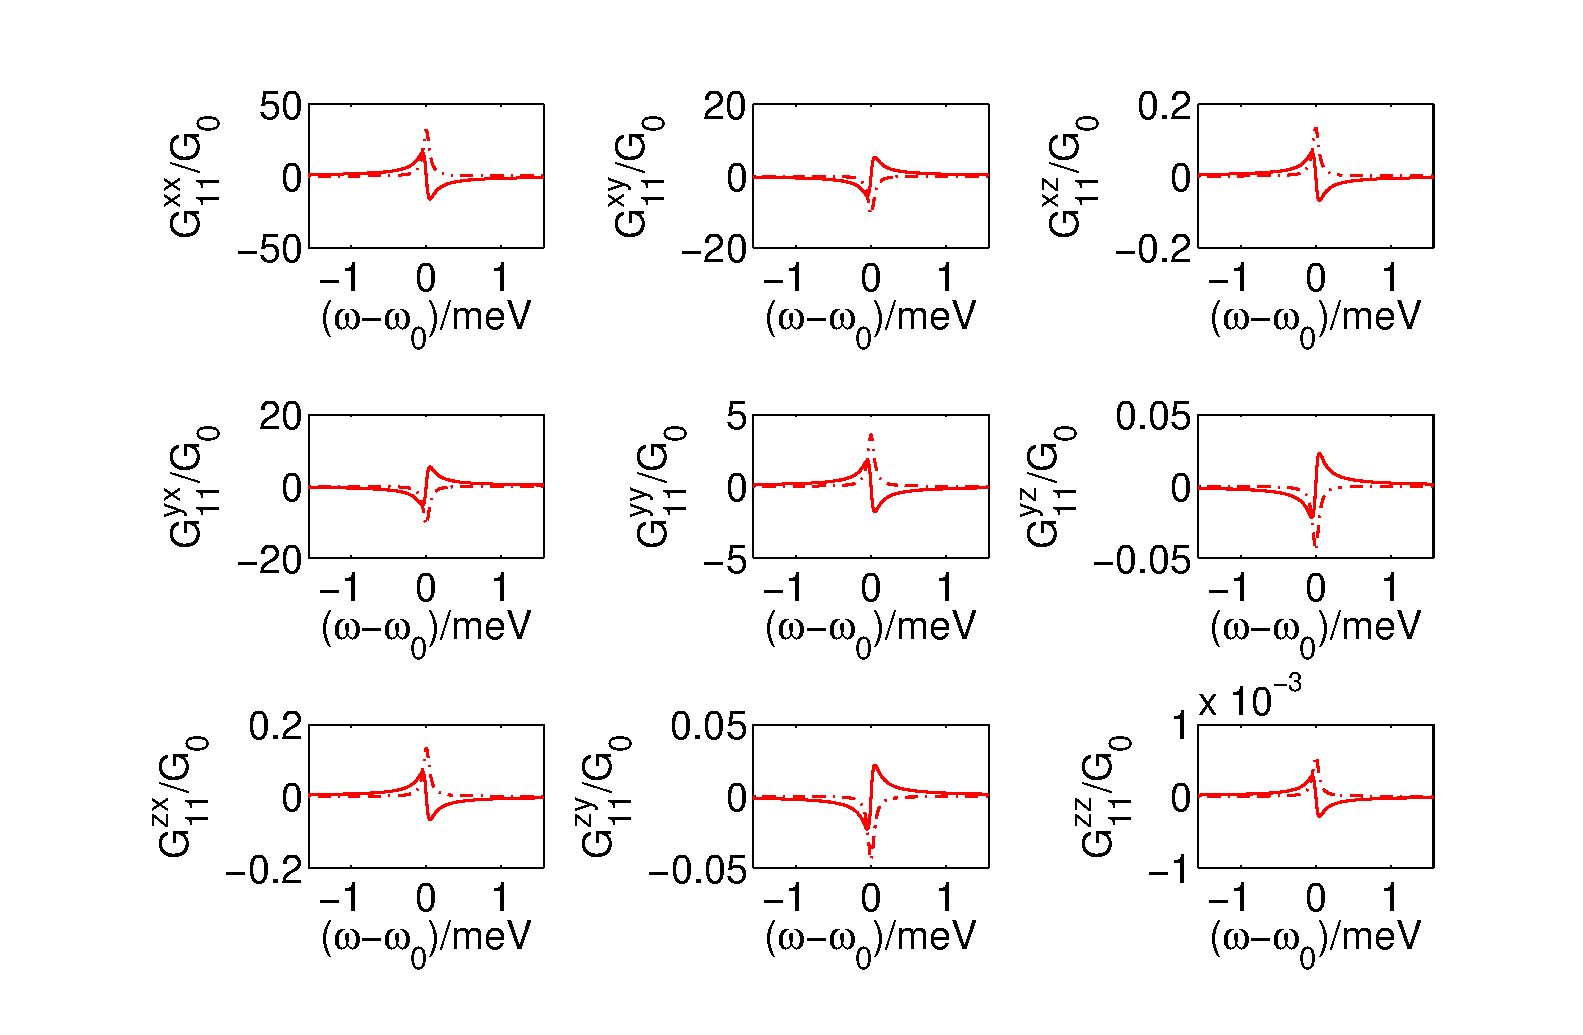
\includegraphics[width=16cm]{./Figs/G84_11_4}
\end{center}
\caption[Full elements of $G^0$ with $\omega_c/2\pi = 317 {\text {THz}} (\lambda_c=945 {\text {nm}}), \Gamma_c = 0.1 {\text {meV}}$]{\textbf{Full elements of $G^0$ with $\omega_c/2\pi = 317 {\text {THz}} (\lambda_c=945 {\text {nm}}), \Gamma_c = 0.1 {\text {meV}}$ }. The source locates at  $\br_1=[60,100\sqrt{3}+60,\, 0]$ nm (see Fig.~\ref{dotsmode1_2}) with both large x and y components of GFT. The $\mathbf{G}^{ij}_{11}$ is the $ij$-th component of the $\mathbf{G}^{(0)}(\br_1,\br_1,\omega)$. Dashed lines are the imaginary part of the GFs; solid lines are the real parts of the GFs. All components are normalized to the homogeneous GF, $G_0$, given by Equ.\eqref{Ghom2}. }
\label{G84_11_4}
\end{figure}

The $yy$ component of the total GFT for this 1-dipole system is shown in Fig.\ref{G84_1yy_2}. Compared with the scalar computational method, which only takes the $yy$ component of $\Gb$ and $y$ component of dipole moment into account, the full tensor calculation shows a cross-coupling effect from the $x$ component.
\begin{figure}[H]
\centering
\begin{center}
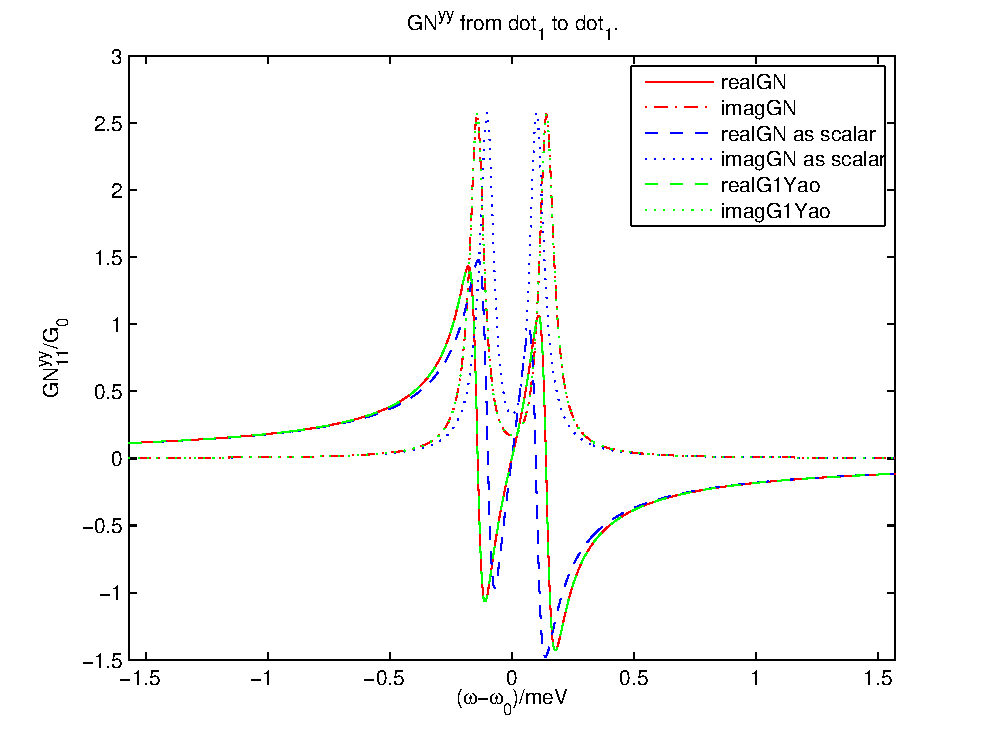
\includegraphics[width=14cm]{./Figs/G84_1yy_2}
\end{center}
\caption[yy component of $G^1(\mathbf{r}_1,\mathbf{r}_1)$  with one on-resonance dipole.]{\textbf{  yy component of $G^1(\mathbf{r}_1,\mathbf{r}_1)$  with one on-resonance dipole}. Red lines show the full tensor calculation of the real and imaginary parts of the yy component at dipole 1; blue lines show the scalar calculation of GF at dipole 1 responding to itself, by only taking the yy component of $\Gb$ and y component of dipole moment into account; green lines show the results of one-dipole GFT with scalar denominator as described in Appendix~\ref{section:GFscalar}~\cite{Yao2009b} for comparison. Now we can see the blue line does not match with other lines. This is because both $yx$ and $xy$ components of $\Gb$ play roles in the GFT calculation, and the tensor algebra cannot be simplified as a scalar algebra since the cross-coupling effect becomes evident. While the red and green lines agree very well. This shows the equivalence of these two theories.}
\label{G84_1yy_2}
\end{figure}

For the cases we have studied in the last subsection above, if the dipole source is polarized to neither $x$ nor $y$ direction, the spectra show that making the denominator to be a scalar in the total GFT expression is equivalent to the full tensor treatment (see Appendix~\ref{section:GFscalar}). As an example to exam different GF calculation methods, the $x$- and $y$-polarized spectra for off- and on-resonance cases are shown in Fig.\ref{sp84_11_7x}, and Fig.\ref{sp84_11_7y}. The plots in the two figures show that the iterative and non-iterative methods and the method presented in Appendix~\ref{section:GFscalar}~\cite{Yao2009b} are equivalent.
\begin{figure}[H]
\centering
\begin{center}
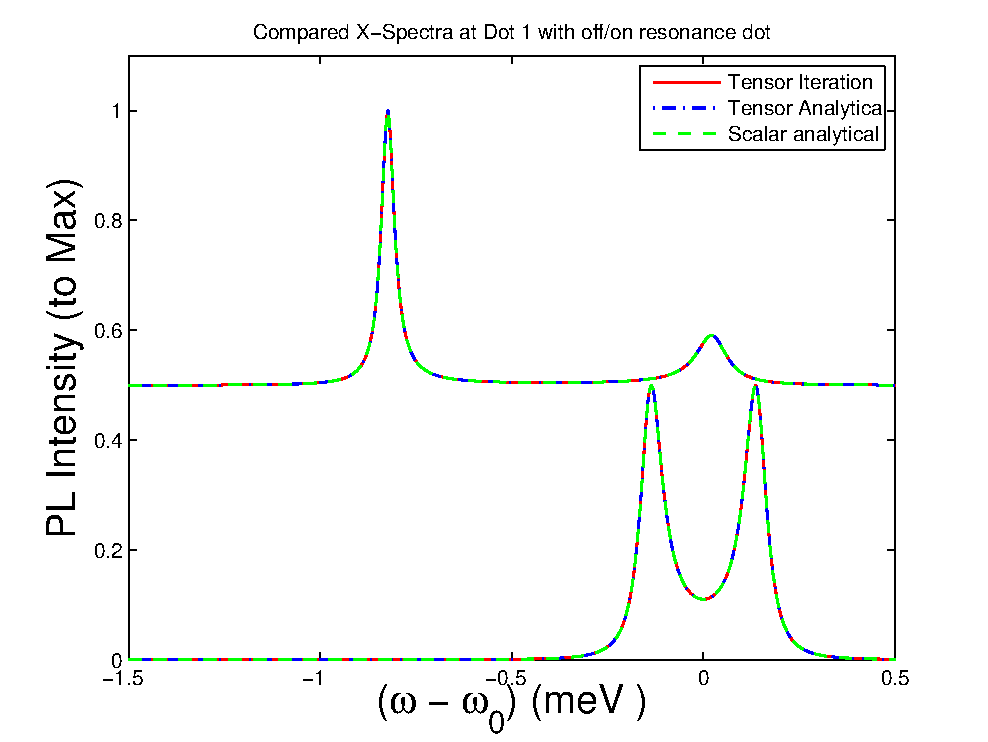
\includegraphics[width=14cm]{./Figs/sp84_11_7x}
\end{center}
\caption[X component of Spectra of off-resonance and on-resonance dipoles.]{\textbf{  X component of Spectra of off-resonance (top) and on-resonance (bottom) dipoles in the PC cavity, detected at the dipole position, with dipole decay rate of $\Gamma_d = 40 \mu{\text {eV}}$ }. Top lines are with a detuning $\Delta \omega = -0.8 {\text {meV}}$. Red lines are obtained through full tensor iteration method; blue lines are obtained through full tensor non-iteration analytical expression in Appendix~\ref{section:noniterativeGF}; green lines are based on the GFT calculation method reported in Ref.~\cite{Yao2009b} or Appendix~\ref{section:GFscalar}. The amplitudes are normalized to the maximum of the absolute value of the PL spectrum. The top curves are offset by 0.5 for clarity.}
\label{sp84_11_7x}
\end{figure}

\begin{figure}[H]
\centering
\begin{center}
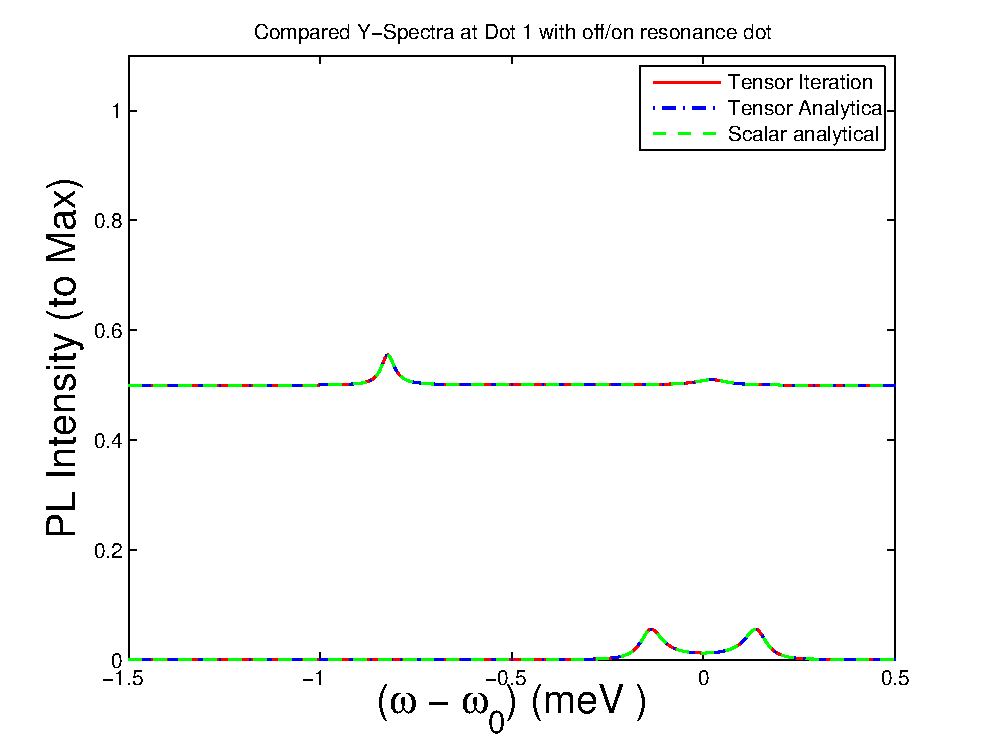
\includegraphics[width=14cm]{./Figs/sp84_11_7y}
\end{center}
\caption[Y component of Spectra of off-resonance and on-resonance dipoles.]{\textbf{  Y component of Spectra of off-resonance (top) and on-resonance (bottom) dipoles in a PC cavity}. Notation and calculation methods are the same as Fig.~\ref{sp84_11_7x}. The top curves are offset by 0.5 for clarity.}
\label{sp84_11_7y}
\end{figure}


%\clearpage

\subsection{Two-dipole coupled cavities}
\subsubsection{Two-dipole system with $y$-polarized sources}
In this part, we will demonstrate the spectrum of the two-dipole coupled cavity.
Results will be compared with those of Ref.~\cite{Yao2009c}.
%The testing code is located at GFT tool box repository/Test with a name SpecPC\_2.m (version 7, but need to change en to be [0,1,0] in the code).
The parameters used are as follows:
%\begin{equation}
\begin{align}
 \omega_c/2\pi = \omega_{1(2)}/2\pi &= 191.551 {\text {THz}},\\
 \Gamma_c &= 20.2 \mu{\text {eV}}, \\
 d_{1(2)} &= 30 {\text {Debye}}, \\
 \Gamma_{d1(2)} &= 2 \mu{\text {eV}}, \\
 g_1 = 0.0564 {\text {meV}}, &\quad g_2=0.0230 {\text {meV}}.
\end{align}
%\end{equation}
These two dipoles are located at $\br_1=[0,0,0]$ nm and $\br_2=[0,190*\sqrt{3},0]$ nm, where the origin is the center of the cavity (Fig.\ref{dotsmode2_1}). We use $\omega_{1 (2)}$ indicating the dipole 1(2)' resonance, which is on-resonance. $d_{1(2)}$ and $\Gamma_{d1(2)}$ are the optical moment and decay rate of dipole 1(2), respectively. $g_1$ and $g_2$ are the coupling strengths of the two dipoles based on Equ.\eqref{eq:g1}. The $yy$ component of the total GFT for this system is shown in Fig.\ref{G84_2yy11_1}. Comparisons among different calculation methods for the spectrum are shown in Figs.~\ref{sp84_11_3} and~\ref{sp84_11_4}. All plots agree with each other very well, and show the splitting feature of the strong coupled dipoles-cavity system.

We notice that, when the two dipoles are both on-resonance, the spectral splitting width is less than $2(g_1+g_2)$, and differs from $2g_1$ or $2g_2$ (see the labels in Figs.~\ref{sp84_11_3} and~\ref{sp84_11_4}). This feature implies that the total coupling strength with two dipoles is not simply the sum of two individual dipole-cavity coupling strengths. Theoretical and experimental studies on identical on-resonance dipoles coupled to a homogeneous field of a cavity confirm that the spectral splitting width are $\sqrt{N}g$, where $g$ is the coupling strength of an individual dipole to the cavity, and $N$ is the number of the dipoles~\cite{Kimble1998,Tischler2007}; in the case above, however, the spectral splitting width cannot be predicted by the $\sqrt{N}g$ relationship, since the dipoles do not share the same coupling strength.  Moreover, we also notice that the splitting width of the spectrum (in Fig.~\ref{sp84_11_3}) is different from that of imaginary part of the GFs ($yy$ component of the $\mathbf{G}^2(\mathbf{r}_1,\mathbf{r}_1)$ in Fig.~\ref{G84_2yy11_1}) as Equ.\eqref{eq:sN_mixedstate_withdecay} defines.
\begin{figure}[H]
\centering
\begin{center}
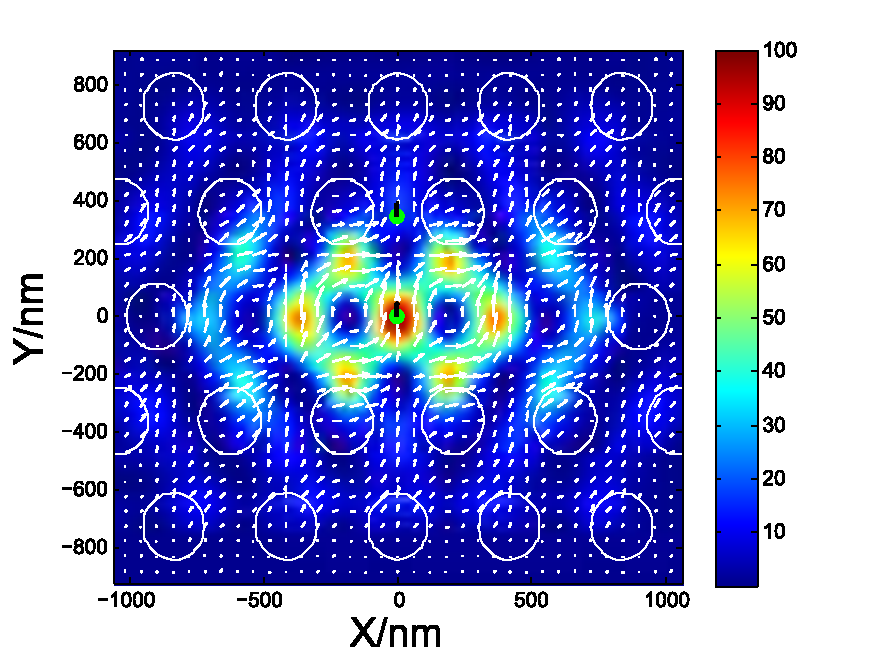
\includegraphics[width=14cm]{./Figs/dotsmode2_1}
\end{center}
\caption[Dipoles and E-field distribution in a H3 PC cavity structure.]{\textbf{  Dipoles and E-field distribution in a H3 PC cavity structure in $z=0$ plane.}  The dipoles (indicated by green points) both polarize in the y direction (see the black arrows), and is located at $[0,\, 0,\, 0]$ nm (the center of the cavity with a strong y-mode) and $[0,\, 190\sqrt{3},\, 0]$ nm. The color map corresponds to the relative strength of the cavity mode. White arrows indicate on-site E-field vectors.}
\label{dotsmode2_1}
\end{figure}


\begin{figure}[H]
\centering
\begin{center}
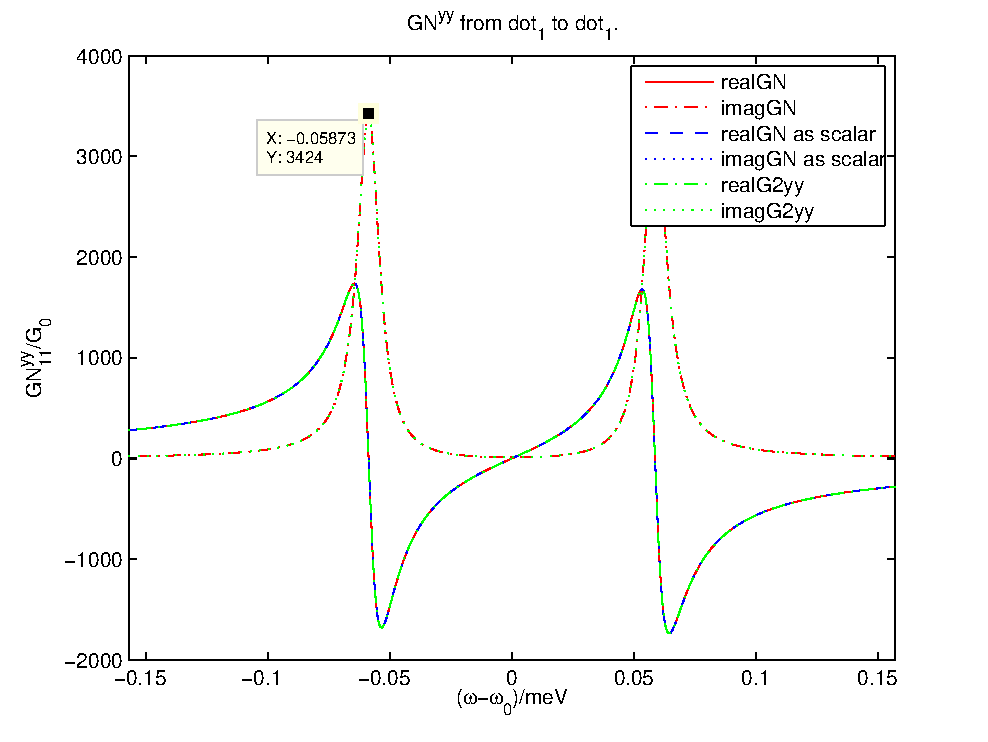
\includegraphics[width=14cm]{./Figs/G84_2yy11_1}
\end{center}
\caption[yy component of $G^2(\mathbf{r}_1,\mathbf{r}_1)$  with two on-resonance dipoles.]{\textbf{$yy$ component of $\mathbf{G}^2(\mathbf{r}_1,\mathbf{r}_1)$  with two on-resonance dipoles of $\Gamma_d = 2 \mu{\text {eV}}$ }. Red lines are obtained by using the full tensor calculation method; blue lines are from the scalar calculation with yy component of $\Gb$ and $y$ component of dipole moment; green lines are the result of the analytical formula in Ref.~\cite{Yao2009c}. These lines are on top of each other. }
\label{G84_2yy11_1}
\end{figure}


\begin{figure}[H]
\centering
\begin{center}
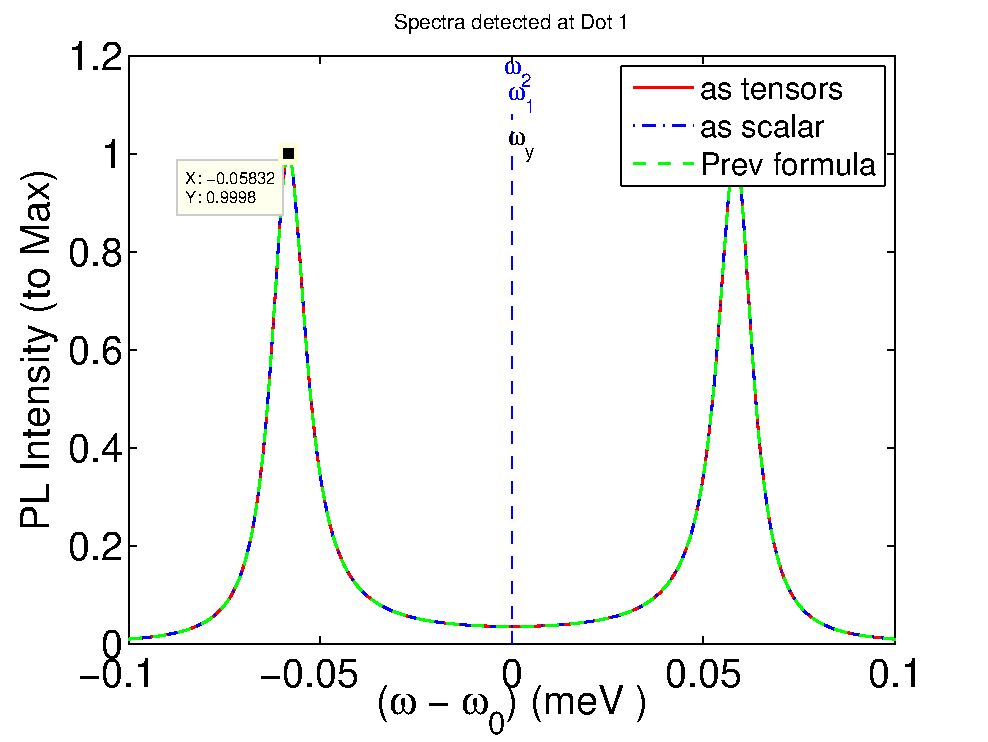
\includegraphics[width=14cm]{./Figs/sp84_11_3}
\end{center}
\caption[Spectra of on-resonance dipoles, with three calculation methods.]{\textbf{Spectra of on-resonance dipoles in a PC cavity, calculated with three methods}. $\omega_y=\omega_0$ is the cavity resonance. Red line is obtained through iterative full tensor method; blue line is obtained through scalar method, by only taking account the $yy$ component of $\Gb$ and $y$ component of dipole moment; green line is the result of the formula in Ref.~\cite{Yao2009c}. These lines are on top of each other.}
\label{sp84_11_3}
\end{figure}


\begin{figure}[H]
\centering
\begin{center}
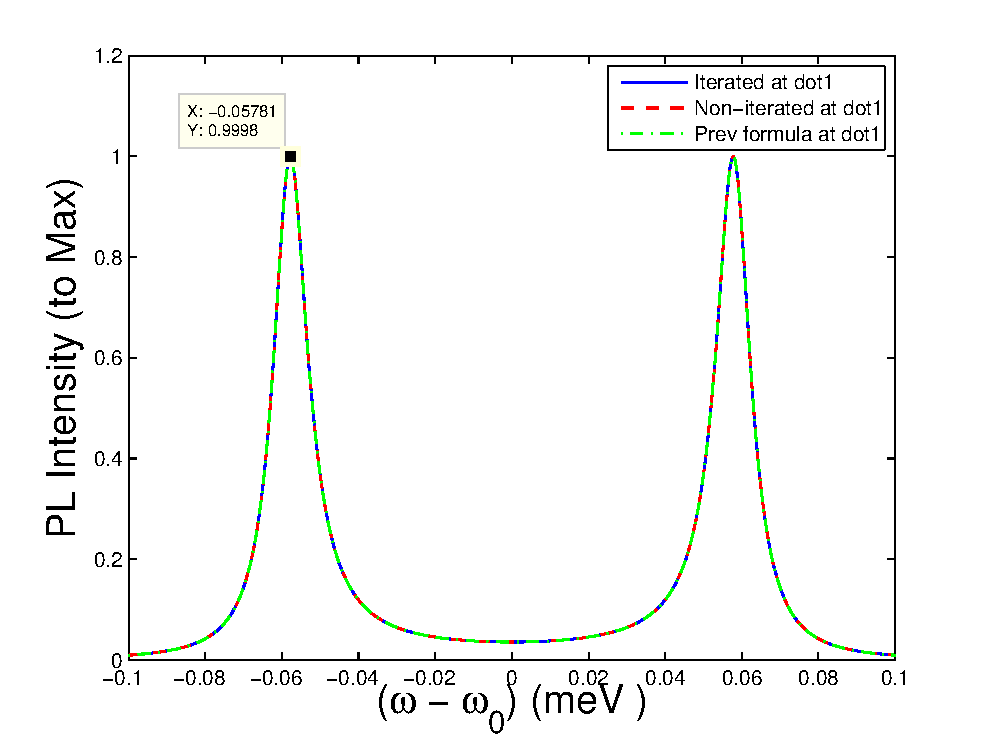
\includegraphics[width=14cm]{./Figs/sp84_11_4}
\end{center}
\caption[Spectra of on-resonance dipoles, based on three analytical expressions.]{\textbf{Spectra of on-resonance dipoles in PC cavity detected at dipole 1 based on three analytical expressions}. Red line is plotted according to full tensor iterative analytical expression in Appendix~\ref{App:GF}; blue line is obtained through non-iterative analytical expression in Appendix~\ref{App:GF}; green line is plotted based on the analytical formula for $G^2$ in Ref.~\cite{Yao2009c}. Again, these three lines are on top of each other.}
\label{sp84_11_4}
\end{figure}

%\clearpage

\subsubsection{Cavity System with Two $xy$-polarized Dipoles}
In this section, we will turn both the dipoles' polarization directions to $45^\circ$ up $x$ axis,
which means the dipoles are polarized between $x$ and $y$ axes.
We locate the dipole sources to places where both $x$ and $y$ components of E-field contribute to the GFT (Fig.~\ref{dotsmode2_2}). Now, the GFT of the bare cavity is non-diagonal (Fig.~\ref{G84_11_2}).
%In this case, we cannot only use $yy$ components of GFTs to analyze the spectrum.
%All graphs in this section are returned from code SpecPC\_2.m version 13 in Test file of GFT project repository.

The $yy$ component of total GFT for this two-dipole system is shown in Fig.~\ref{G84_2yy11_2}. Comparisons of spectra calculated from different methods are shown in Figs.~\ref{sp84_11_5} and~\ref{sp84_11_6}. Again, the cross-coupling effect of the $x$ and $y$ components is evident.

We also notice that the coupling strengths of the two dipoles are $g_1=0.0268$ meV and $g_2=0.0363$ meV; the width of the splitted spectral peaks when the two dipoles are on-resonance is $2\times 0.01107$ meV, which is less than both $2g_1$ and $2g_2$. Similar to the solely $y$-polarized case discussed in the last subsection, again, we observed the complicated combination of two dipoles coupling to a cavity. In both cases, we employed the separation of doublets to be the spectral splitting width. In Chapter~\ref{ch:ensemble}, we will use the FWHM as the general description quantity to measure how the spectrum is broadened or narrowed.

The spectral behaviors (shifting and broadening) with more than two dipoles will be discussed in the next section and the next chapter.
\begin{figure}[H]
\centering
\begin{center}
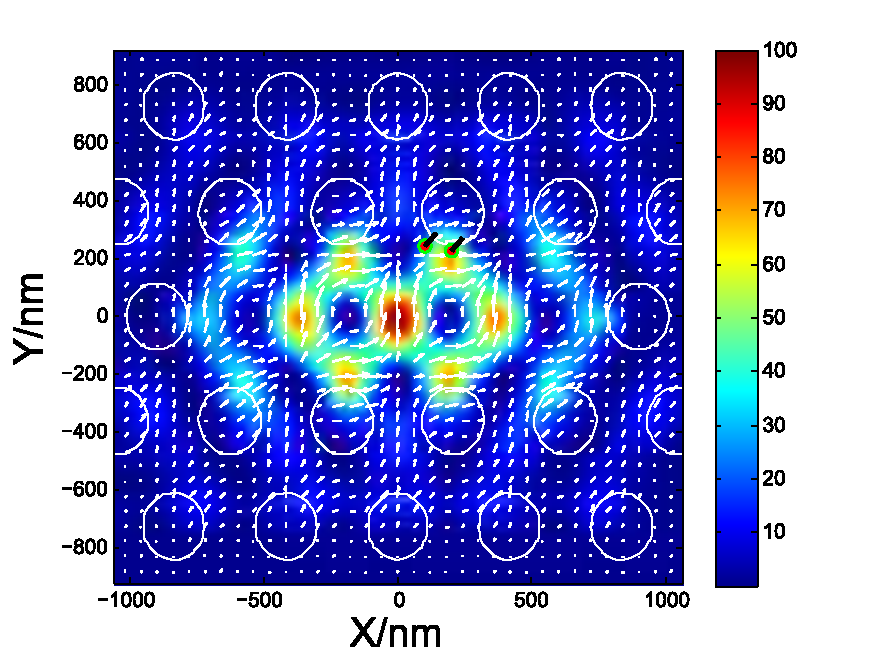
\includegraphics[width=14cm]{./Figs/dotsmode2_2}
\end{center}
\caption[Dipole and E-field distribution in a H3 PC cavity structure.]{\textbf{  Dipoles and E-field distribution in a H3 PC cavity in the $z=0$ plane.}  The dipoles (red points) polarize to x-y direction (see the black arrows at the dots) and locate at $\mathbf{r}_1=[100,\, 240,\, 0]$ nm and $\mathbf{r}_2=[200,\, 100\sqrt{3}+40, \, 0]$ nm, where the E-fields have both x and y components. Color map corresponds to relative strength of the cavity mode, and white arrows indicate on-site E-field vectors.}
\label{dotsmode2_2}
\end{figure}

\begin{figure}[H]
\centering
\begin{center}
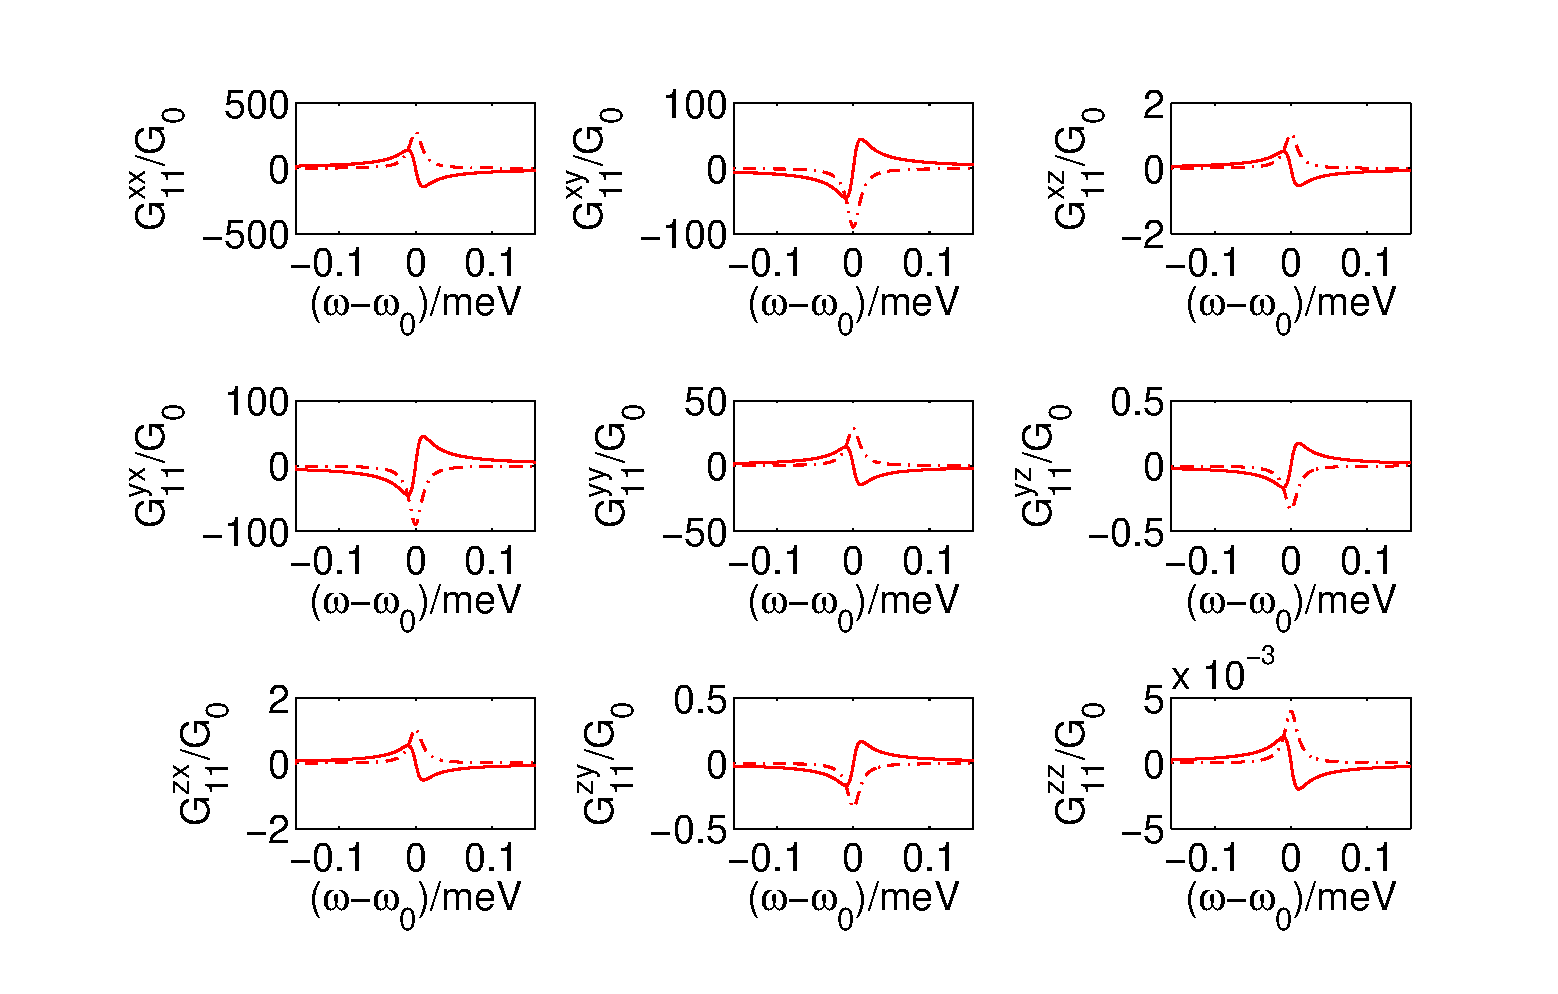
\includegraphics[width=16cm]{./Figs/G84_11_2}
\end{center}
\caption[Full elements of $G^0(\mathbf{r}_1,\mathbf{r}_1)$.]{\textbf{Full elements of $G^0(\mathbf{r}_1,\mathbf{r}_1)$. $\omega_c/2\pi = 191.155 {\text {THz}},\, \Gamma_c = 0.010 {\text {meV}}$ }. The $\mathbf{G}^{ij}_{11}$ is the $ij$-th component of the $\mathbf{G}^{(0)}(\br_1,\br_1,\omega)$. Dashed lines are the imaginary part of the GFs; solid lines are the real parts of the GFs. All components are normalized to the homogeneous GF, $G_0$ (Equ.\eqref{Ghom2}).}
\label{G84_11_2}
\end{figure}


\begin{figure}[H]
\centering
\begin{center}
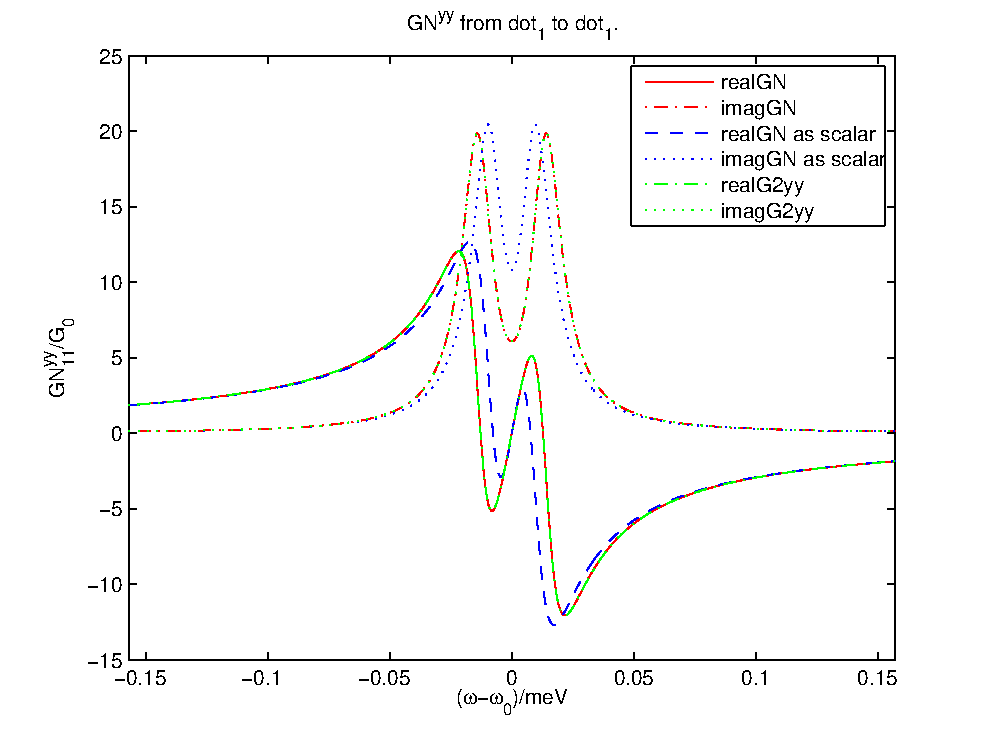
\includegraphics[width=14cm]{./Figs/G84_2yy11_2}
\end{center}
\caption[yy component of $G^2(\mathbf{r}_1,\mathbf{r}_1)$  with two on-resonance dipoles.]{\textbf{  yy component of $G^2(\mathbf{r}_1,\mathbf{r}_1)$  with two on-resonance dipoles. $\Gamma_d = 2 \mu{\text {eV}}$ }. Red lines show the full tensor calculation result; blue lines show the scalar calculation result; green lines are from the analytical formula in Ref.\cite{Yao2009c}. The blue line does not agree with others. This is because the bare cavity GFT cannot be simplified as a scalar. The red and green lines match up perfectly.}
\label{G84_2yy11_2}
\end{figure}


\begin{figure}[H]
\centering
\begin{center}
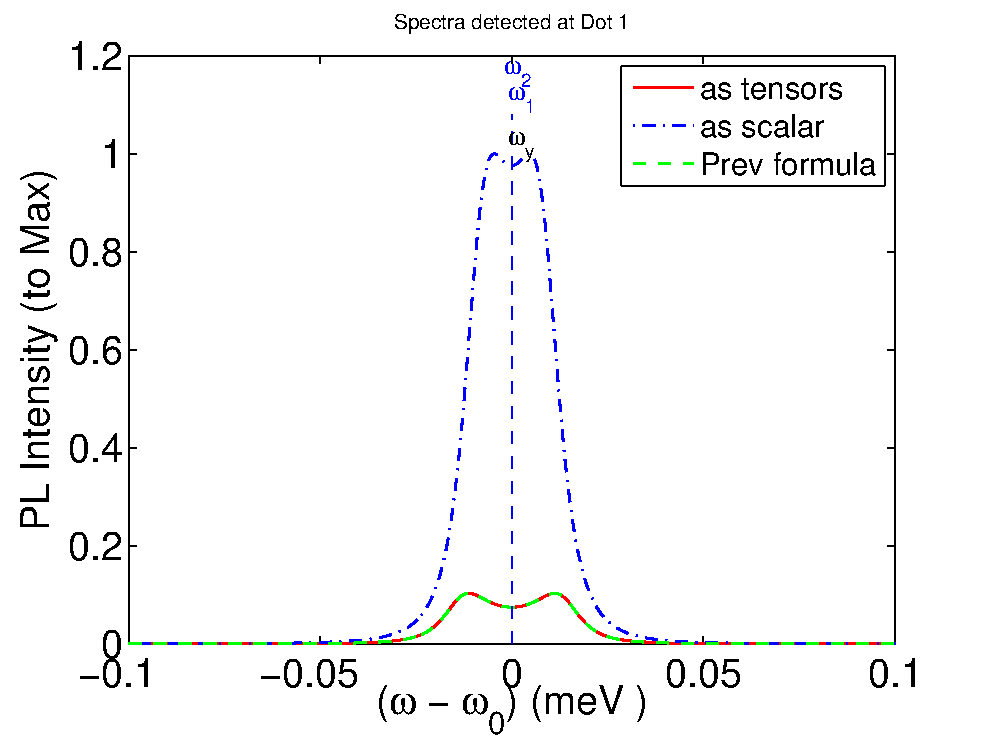
\includegraphics[width=14cm]{./Figs/sp84_11_5}
\end{center}
\caption[Spectra of on-resonance dipoles, with three calculation method.]{\textbf{Comparison of three calculation methods for the spectra with two on-resonance dipoles in a PC cavity.} Red line is obtained through full tensor method; blue line is obtained through only taking the yy component of the bare cavity GFT and the y component of the dipole moment into account; green line is from the analytical formula in Ref~\cite{Yao2009c} by making the denominator a scalar. Except for the blue line, other lines agree with each other perfectly. Lines are normalized to the maximum of the blue line.}
\label{sp84_11_5}
\end{figure}


\begin{figure}[H]
\centering
\begin{center}
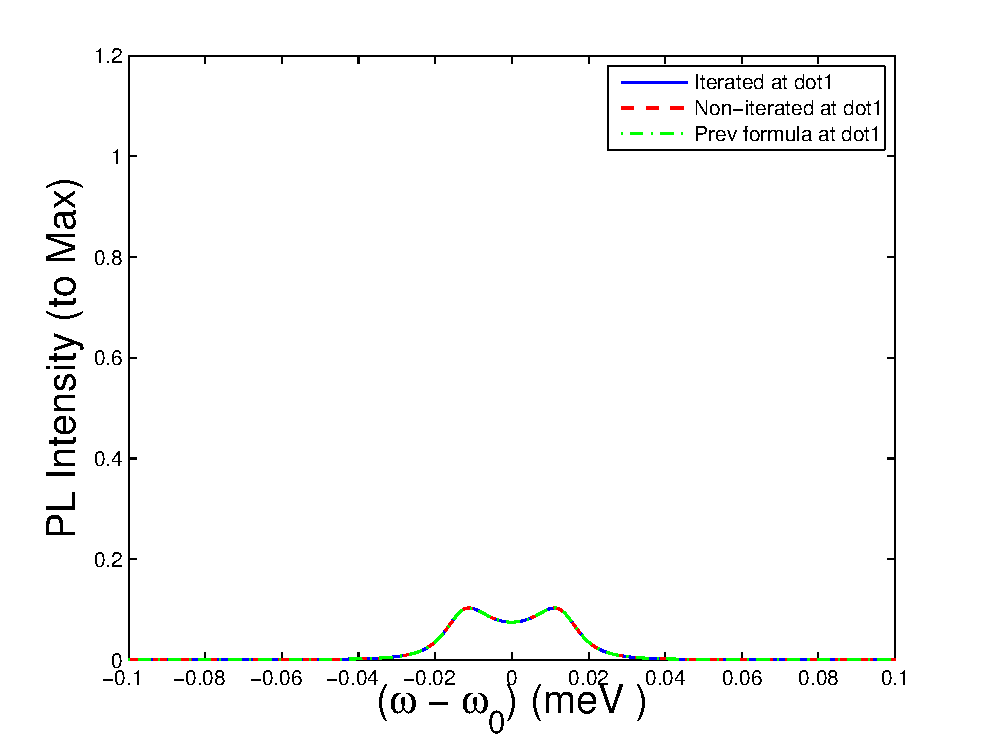
\includegraphics[width=14cm]{./Figs/sp84_11_6}
\end{center}
\caption[Spectra of on-resonance dots, based on three analytical expressions.]{\textbf{Comparison of spectra of on-resonance dipoles in a PC cavity from three analytical expressions}. The red, blue and green lines are obtained from the full tensor iterative, non-iterative analytical expressions (Appendix~\ref{App:GF}) and the analytical formula in Ref~\cite{Yao2009c}, repectively. These three lines agree with each other very well. With the same scale as Fig.~\ref{sp84_11_5}.}
\label{sp84_11_6}
\end{figure}

\subsection{Summary}
In this section, we studied the cavity spectral behaviors under the interaction with one or two dipoles. We observed a slight spectral shift effect in the presence of dipoles. We also observed the spectrum is affected by the width, coupling strength and position of the dipoles. Especially, when there are more than one dipoles in the cavity, the spectrum is complicated. As an example, the on-resonance two dipoles coupled cavity is studied in detail.

As have been demonstrated in this section, the $z$-components of GFTs for this PC cavity are always negligible. Moreover, once the dipole moments and the E-field are aligned in the same direction and on either $x$- or $y$-axis, there is no cross-coupling effect on $x$ and $y$ components of the GFTs and spectra; otherwise, the cross-coupling effect between $x$ and $y$ components takes place so that one cannot only use the diagonal elements of the bare cavity GFT to calculate the cavity spectrum with dipoles.

From now on, we will focus on the collective emitting effect, and leave the detailed discussion on the cross-coupling effect as a future work.

\section{Multiple Dipoles Coupled to a PC Cavity}\label{PCcase}
In general, a system of two coupled oscillators has two eigenfrequencies~\cite{Goldstein2002}. As the coupling strength increases, the lower eigenfrequency decreases and the higher one increases; this is a ``repulsion'' effect between the eigenfrequencies. The quantum mechanical analog of this repulsion effect is known as the Wigner-Von Neumann anticrossing rule~\cite{Neumann1929,R.P.Feynman1970, C.Cohen-Tannoudji1977, Frank1994}. Examples include the hyperfine splitting of the hydrogen atom in a magnetic field~~\cite{R.P.Feynman1970}, the neutrino oscillation between flavors~\cite{Sassaroli1999}, the Nilsson model for deformed nuclei~\cite{Ring2004}, and RLC circuits resonators repulsion~\cite{Gamarra2007}. The nonlinearly increased repulsion as the frequencies separation of two resonators decreases. As well, the non-Lorentzian distribution of ensemble resonances, will lead to inhomogeneous spectral reshaping, as will be discussed later.

In this section, we will fully calculate the spectrum of a practical low-density-dipole coupled PC cavity,
in which the frequency repulsion effect and the inhomogeneous coupling effect will be highlighted as a bridge to the next chapter.

Now, we randomly distribute 41 QDs in a H3 PC cavity slab~\cite{Akahane2003} with an non-radiative decay rate ($\Gamma_c$) of $0.1$ meV,
and randomly orientate their polarization directions in the $x-y$ plane.
The QD labeled No.1 is at the center of the cavity and oriented in the $\pm y$ direction.
All QDs share the same dipole moment of $50$ Debye,
which gives QD 1 the largest coupling strength of $0.1$ meV among all the other QDs.
The locations and orientations of all QDs are shown in Fig.\ref{QDmode} in the background of cavity mode distribution in the PC slab.
We have used a commercial FDTD software from Lumerical Solutions~\cite{LumericalSolutions} and house-made codes to calculate the cavity mode.
Notice that, in this section, we have supposed there is only one dipole excited for every QD,
and all QDs are laid in a $\pm1000 {\text nm} \times \pm1000 {\text nm}$ area around the cavity center.
We also assign the QDs sample's resonances with a Gaussianly distributed statistical profile centered at $-5$ meV lower to the cavity resonance which is $792.25$ meV.
Every QD has a decay rate ($\Gamma_d$) of $0.05$ meV.
The spectrum is detected in the y-direction for these QDs in a homogeneous medium is shown in Fig.~\ref{QDspecPChom}(a).
%We can see that the relative strengths of the QDs in $y-$direction are correlated with their polarization directions, which determines the projection of dipole moment on the given polarization direction.
\begin{figure}[htp]%[floatfix]
\centering
\begin{center}
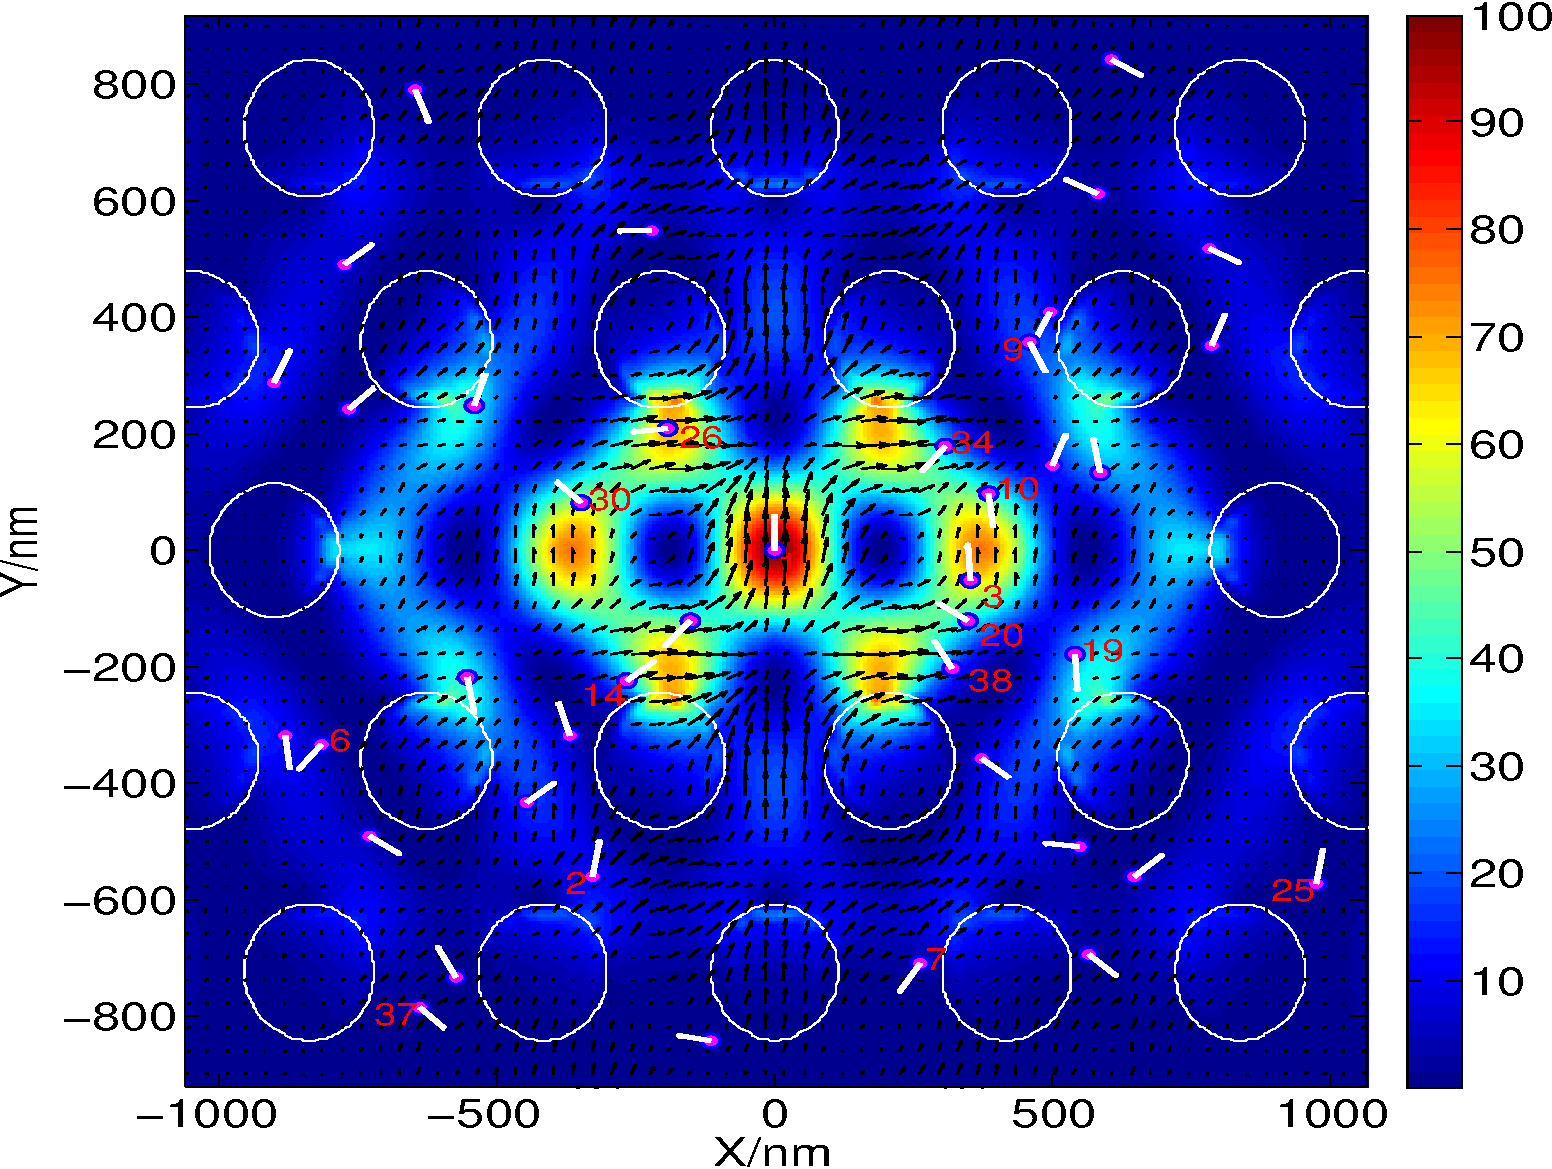
\includegraphics[width=12cm]{./Figs/QDmode}
\end{center}
\caption[Cavity mode and 41-QD distribution in a PC cavity.]{\textbf{  Cavity mode and QDs distributions map.} The background color map shows the electrical field strength, with black arrows indicating the field directions. The pink dots with white tails indicate the position and oscillating directions of the QDs. Numbers nearby the QDs are the labels for interested QDs. }
\label{QDmode}
\end{figure}



\begin{figure}[htp]%[floatfix]
\centering
\begin{center}
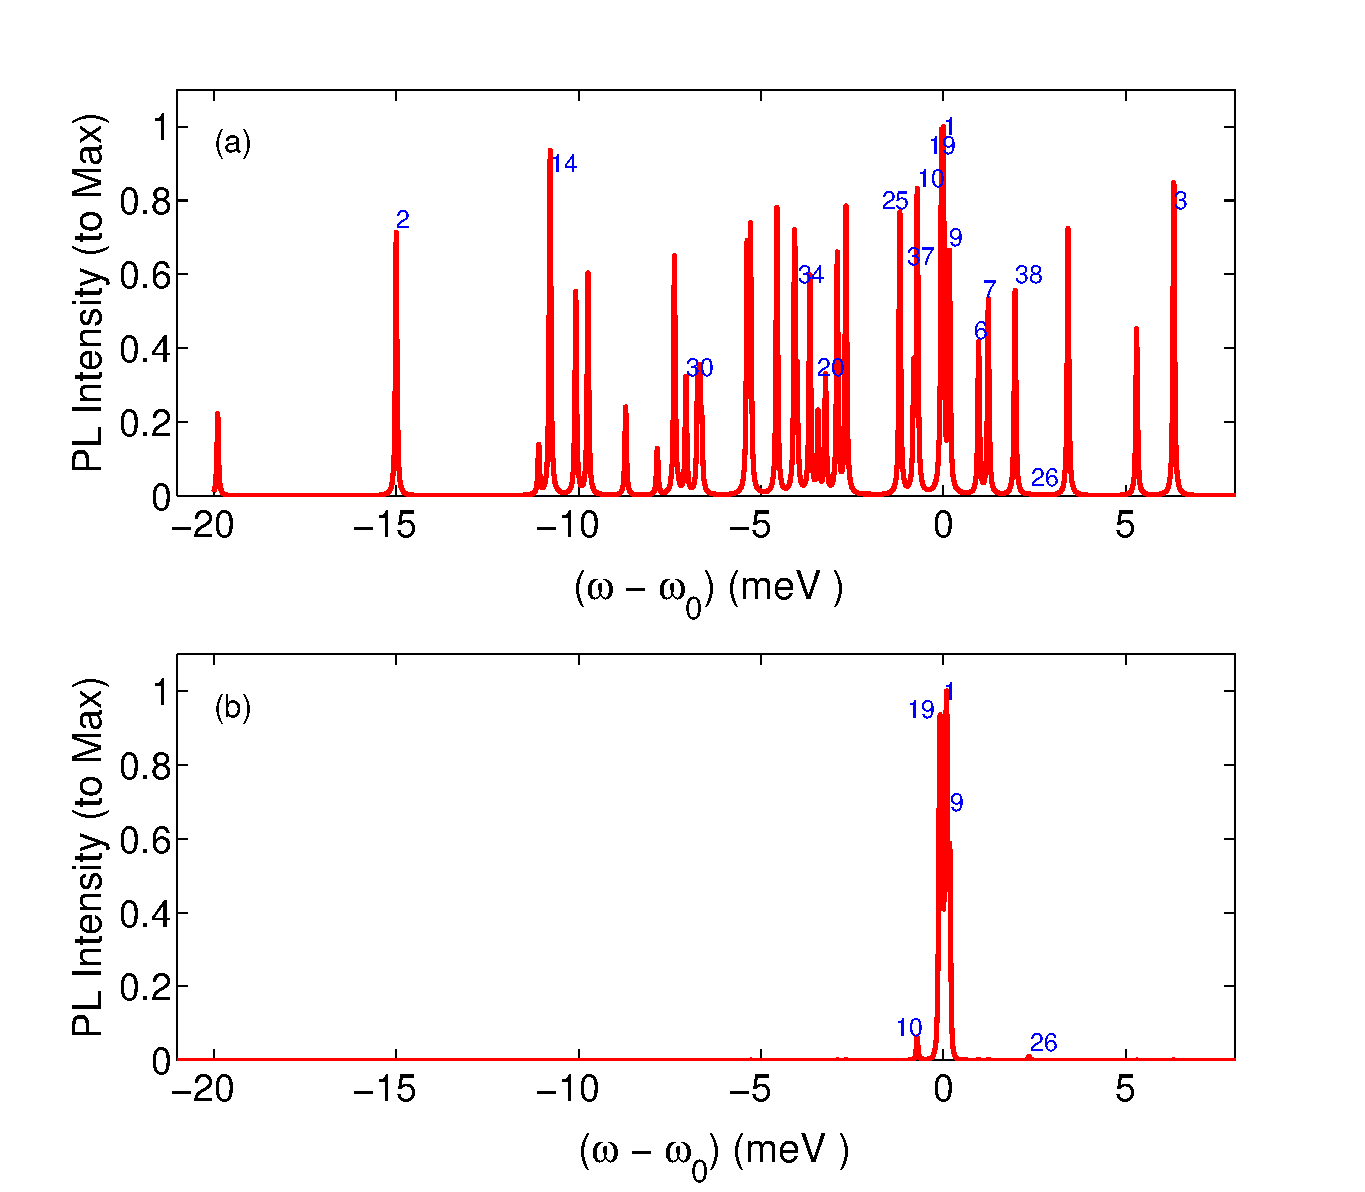
\includegraphics[width=12cm]{./Figs/QDspecPChom}
\end{center}
\caption[Spectra of 41 QDs in a homogeneous medium and a PC cavity.]{\textbf{$Y$-polarized Spectra of 41 QDs in a homogeneous medium (a) and the PC cavity (b).} The QDs ensemble has a Gaussian distribution profile, centered at 5 meV lower than the cavity mode resonance, with standard deviation $\sigma=20$ meV. Numbers around the peaks indicate the corresponding QDs' label. QD 1 is on resonance at $\omega_0$, nearby QDs to the low frequency side are QDs 19 and 10, to the high frequency side are QDs 9 and 26, in the bottom figure.}
\label{QDspecPChom}
\end{figure}

While coupled to the cavity mode, the QD peaks resonating far away from the cavity resonance are washed out, only leaving the cavity peak along with a few QDs peaks either close to the cavity resonance or at strong field positions (see Fig.~\ref{QDspecPChom}(b)).
This result shows that three factors can make the QD peaks visible in a coupled system.
One is the local field strength, and another is the magnitude of dipole moment projected on local field direction.
These two factors, multiplied together, give the coupling strength of the QD to the cavity.
The last factor is the related position of QD's resonance to the cavity resonance.
The closer these two resonances are, the larger the spectral peak occurs.
This factor shows an inhomogeneous enhancement of spectral formation in oscillators coupling.
In sum, the coupling strength and resonance positions will greatly affect the cavity optical property.
%We will discuss the two factors in the following sections.

As we will see, the relative positions of the dipole resonances and the cavity resonance can give various spectral effects, including frequency repulsion, attraction, splitting, screening effects and so on. We would like to give a brief visualization of these effects, as they are the foundation for our discussion on dense-dipole coupled systems. As follows, we will discuss the frequency repulsion, splitting and screening effects by shifting the resonance of the No.1 QD from $+0.6$ meV to $-0.6$ meV around the cavity resonance, while keeping all the other QDs in the PC slab as before. The spectrum is shown in Fig.~\ref{QDwd1shift}.
As we can see, when QD 1 is on the high frequency side of the cavity resonance ($\Omega_1-\omega_0>0$), the observed QD 1 peak (see the wave envelope around the blue dashed line) is on the high frequency side of the intrinsic resonance position where it's supposed to be (marked with blue dashed line in Fig.~\ref{QDwd1shift}). The cavity peaks (two or three peaks very close to the cavity resonance are combined as cavity peaks in this discussion) is enhanced on the far side to $\Omega_1$, while the cavity coupled peaks close to $\Omega_1$ are suppressed. A similar effect occurs when the QD 1 is on the low frequency side of the cavity resonance. The displacements of the dipole and cavity peak show the frequency repulsion effect introduced earlier. If $\Omega_1=\omega_0$, the cavity shows a doublet (here, $g_1>\Gamma_1$), which illustrates the establishment of the strong coupling effect between QD 1 and the cavity and gives the spectral splitting effect. One may have also noticed that there is a small dipole peak (labeled as QD 19, close to the cavity resonance) merging in the cavity peak and basically keeps it stable, regardless of the moving of QD 1 in frequency domain. This stability of the dipole peak in a cavity peak can be called screening effect.

One can find that the closer QD 1 is to the cavity resonance, the larger the repulsion effect becomes (for example, by comparing the QD 1 shifts of the observed peak to its intrinsic resonance between occasions of $\Omega_1=\omega_0+0.6$ meV and $\Omega_1=\omega_0+0.4$ meV). The same applies to the dipole-dipole coupling. If we compare the offset of QD 1 peak to its original resonance at $\Omega_1=\omega_0-0.6$ meV and $\Omega_1=\omega_0+0.6$ meV, we find that the former one is smaller than the latter one, because in the former case, there is a QD 10 coupling to QD 1 as well, which also generates a repulsion effect for the QD 1 peak in the opposite direction to cancel a part of the repulsion effect from the cavity peak. However, the repulsion effect from QD 10 to QD 1 is not strong enough to totally cancel the repulsion from the cavity, as the field strength at QD 10 is much smaller than that at QD 1. The amplitude changes obey the same rule as the shifts. One can find that QD closer to the cavity resonance can give larger influence on the cavity peaks compared to the far-off-resonance cases. In the case of discrete dipoles in coupled cavities, if a dipole is too far away from the cavity resonance (dipoles outside of the calculation range in Fig.~\ref{QDwd1shift}, for example), its influence is negligible. This resonance distance related enhancement effect can be called as inhomogeneous enhancement effect.

%This inhomogeneous enhancement effect will also be discussed for the dense dipoles coupled cavities later.

%The other phenomenon we can see in the process is inhomogeneous enhancement of coupling. We can see that when $\omega_1$ is far off the cavity resonance, the QD 1 peak is relatively smaller than the case when $\omega_1$ is close to the cavity resonance, compared to the maximum value of the spectrum. Compared with the peak height of QD 10 sitting at the position where the cavity peaks raise little effect on it, if we look at the cases when QD 1 is not in the left side of the cavity resonance, we can conclude that the maximum value of the cavity peaks is much larger when QD 1 is close to it than the opposite cases. What's more, the QD 19 and QD 9, which are close to the cavity resonance, can give large peaks even when all other QDs are far away from them. In sum, we can conclude that the near-on-resonance QDs can give larger contribution to the cavity spectrum, and hence can change the cavity's optical property much more than that are far away from the cavity resonance. We will discuss the inhomogeneous broadening effects further in the following sections.

\begin{figure}[htp]%[floatfix]
\centering
%\begin{center}
\subfigure[ ]{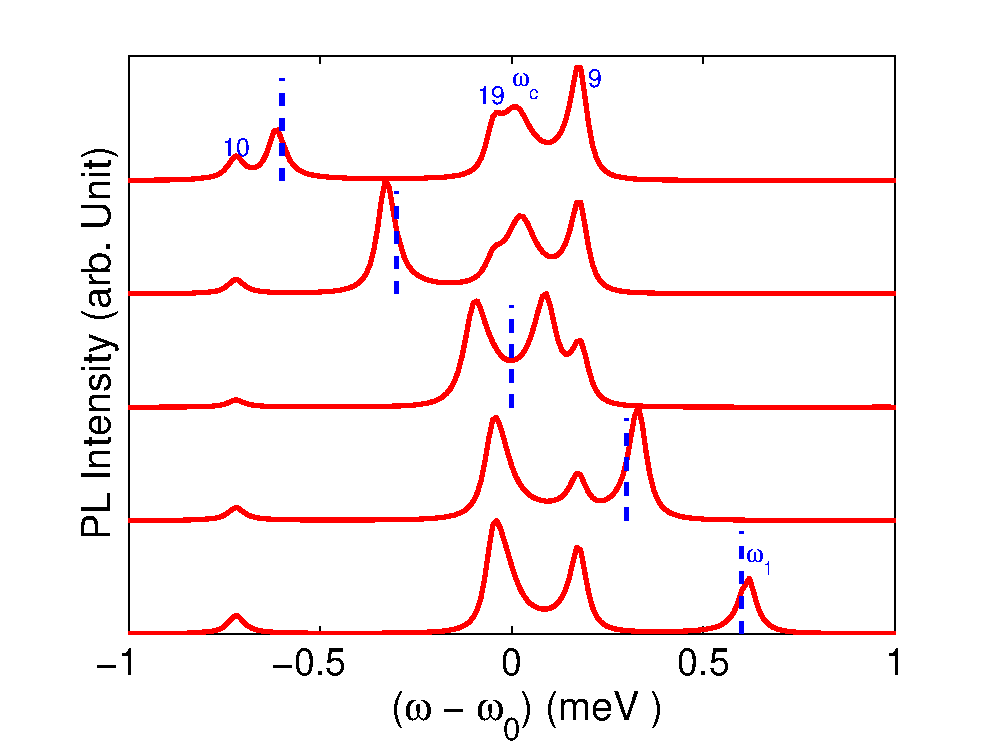
\includegraphics[width=0.46\textwidth]{./Figs/QDwd1shift}
%\end{center}
%\caption{\textbf{Spectrum changes as Dot1 moves around.} The QDs ensemble has a Gaussian distribution profile, centered at 5 meV left to cavity mode resonance, with standard deviation $\sigma=20$ meV. }
  \label{QDwd1shift}}
%\end{figure}
%\begin{figure}[floatfix]
%\centering
%\begin{center}
\subfigure[ ]{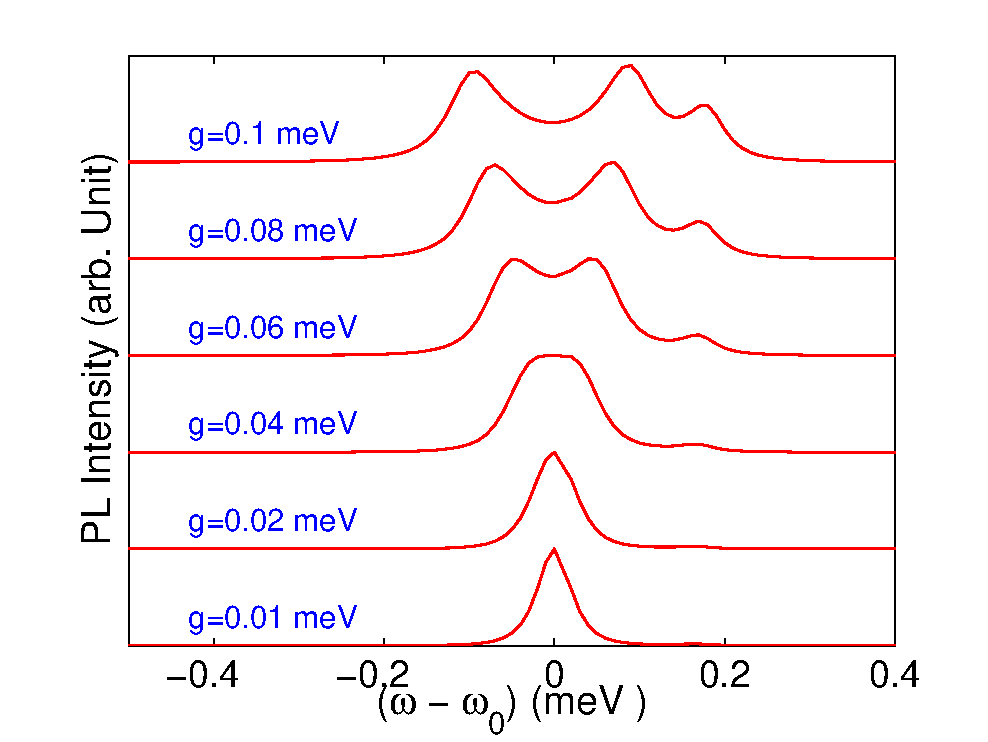
\includegraphics[width=0.46\textwidth]{./Figs/QDdetuneg}
  \label{QDdetuneg}}
%\end{center}
\caption[Cavity Spectra as QD 1 shifts and the coupling constant changes.]{\textbf{Cavity Spectra as the frequency of QD 1 shifts (a) and the coupling constant changes (b).} In \subref{QDwd1shift}, the QD 1 frequency moves from $+0.6$ meV to $-0.6$ meV from bottom to top in steps of $0.3$ meV.
% inhomogeneous coupling and frequency repulsion effects occur (see text). \subref{QDdetuneg} shows, as the coupling strength of QD 1 changes from $0.01$ meV through $0.04$ meV to $0.1$ meV, the cavity shows the Purcell effect, which has a narrower spectrum than $0.1$ meV, and strong coupling effect, which shows a resonances splitting and broadening effects.
 }
\end{figure}

Experimentally, one can tune the resonance of a QD by changing the temperature, and observe the frequency repulsion and inhomogeneous enhancement effects in cavities (see, for example, Refs.~\onlinecite{Reithmaier2004,Reitzenstein2006}). The cavity shifts and enhancement can be easily observed experimentally, since the intrinsic resonance of the cavity is basically static with changing temperature. For the QD's resonance, however, it is only through a careful calculation, as we performed above, can one notice the slight repulsion effect.

To examine how coupling strength matters, one can tune the coupling strength between the QDs and the cavity by changing the optical moments of the dipoles while fixing the QD 1 on-resonance to the cavity. The spectral changes are shown in Fig.~\ref{QDdetuneg}. We can see that the doublet occurs when the critical condition for strong coupling is satisfied, which is $g_1>\frac{1}{2}\Gamma_c=0.05$ meV for the one-exciton case~\cite{Kimble1998}. If $g_1<0.5$ meV, the QD 1 is in a weak coupling regime to the cavity, which means there is a spontaneous enhancement caused by the Purcell effect~\cite{Purcell1946,G'erard1998}. We will discuss this effect in the context of dense dipoles coupled cavities in the next chapter.



%     \begin{Listing}[H]
%     \filein{Examples/List.als}
%     \caption{Alloy specification of a singly-linked list using only binary relations}
%     \label{list:SimpleList1}
%     \end{Listing}
%
%
% \subsection{Phase 1: High-Level Static Mapping}\label{sec:phase1}
%
%     ...Phase 1 simply generates the default static
%     mapping and presents it to the user, as shown in Figure~\vref{fig:defaultMap}.  We
%     have modified the map file as shown in Figure~\vref{fig:fixedMap}.
%
%     \begin{figure}[H]
%     \begin{singlespacing}
%     \centering
%         \subfigure[Default static mapping]{
%             \begin{minipage}{2.25in}\footnotesize
%                 {\texttt{List = List\\
%                 List\$first =
%                 List.first\\
%                 Node = Node\\
%                 Node\$next = Node.next\\
%                 }
%                 }\label{fig:defaultMap}
%             \end{minipage}}
%         \subfigure[Modified static mapping]{
%             \begin{minipage}{2.25in}\footnotesize
%                 {\texttt{List = SimpleList\\
%                 List\$first = SimpleList.first\\
%                 Node = Node\\
%                 Node\$next = Node.next\\
%                 }
%             }\label{fig:fixedMap}
%             \end{minipage}}
%     \caption[Excerpt of high-level static mapping file]{Excerpt of high-level static
%     mapping file before and after modification}
%     \end{singlespacing}
%     \end{figure}
%
%
%
%     Figure~\vref{fig:tree_beforeAndAfter} shows the tree
%     before and after deletion, with correctly implemented code.
%     Figure~\vref{fig:tree_commentedOut_mainBody} shows the tree after deletion of the
%     root, when the \texttt{root = n2} statement is not executed.
%
%     \begin{figure}[H]
%     \centering
%     \mbox{
%         \subfigure[Before deletion]{\includegraphics[scale=0.65]{Figures/correct_pre}}\label{fig:tree_correct_pre}
%         \subfigure[After correct deletion]{\includegraphics[scale=0.65]{Figures/correct_post}}\label{fig:tree_correct_mainBody}
%         }
%     \caption[Visualization of tree]{Visualization of tree before and after correct deletion of the root node}
%     \label{fig:tree_beforeAndAfter}
%     \end{figure}
%
%     \begin{singlespacing}
%     \begin{figure}[H]
%     \centering
%     \includegraphics[scale=0.75]{Figures/commentedOutWithBetterNumber_post}
%     \caption[Visualization of tree after deletion of root (error or omission)]{Visualization of tree
%     after deletion of the root node, with an error of omission in the code.
%     \texttt{Node\_7} represents the temporary node in the \texttt{swapNodes()} method.}
%     \label{fig:tree_commentedOut_mainBody}
%     \end{figure}
%     \end{singlespacing}
